% MA thesis manuscript: revised version incorporating Megan's feedback (see "MA thesis feedback.md").
% The previous version is manuscript.tex. Visible red [...] placeholders mark text still to be written.
%
% Tables, figures and in-text numbers are read from output/, which is generated by the R scripts in
% code/ (run code/run_all.R from the project root). Compile with pdfLaTeX (Overleaf's default
% compiler); Overleaf runs biber for the bibliography automatically.

\documentclass[12pt, letterpaper]{article}

%---------------------------------------------------------------------------------------------------
% Page layout and spacing
%---------------------------------------------------------------------------------------------------

\usepackage[margin=1in]{geometry}
\usepackage{setspace}                   % 1.5 spacing is switched on after the title and abstract pages
\setlength{\emergencystretch}{3em}      % avoid overfull lines

%---------------------------------------------------------------------------------------------------
% Fonts: Times for text and maths
%---------------------------------------------------------------------------------------------------

\usepackage{amsmath}                    % load before newtxmath
\usepackage[T1]{fontenc}
\usepackage{newtxtext}
\usepackage{newtxmath}
\usepackage{microtype}

%---------------------------------------------------------------------------------------------------
% Lists: no extra space around or between items
%---------------------------------------------------------------------------------------------------

\usepackage{enumitem}
\setlist{topsep=0pt, partopsep=0pt, itemsep=0pt, parsep=0pt}

%---------------------------------------------------------------------------------------------------
% Figures and tables
%---------------------------------------------------------------------------------------------------

\usepackage{graphicx}
\usepackage{float}                      % [H] placement
\usepackage{caption}
\usepackage{subcaption}                 % subfigure environment
\usepackage{booktabs}                   % \toprule, \midrule, \bottomrule
\usepackage{array}                      % >{...} column formats
\usepackage{tabularx}                   % full-width tables with a wrapping column

%---------------------------------------------------------------------------------------------------
% Bibliography: Chicago author-date
%---------------------------------------------------------------------------------------------------

\usepackage[english]{babel}
\usepackage{csquotes}
\usepackage[authordate, backend=biber, compresspages, footmarkoff]{biblatex-chicago} % footmarkoff keeps standard footnote marks
\addbibresource{bibliography.bib}

% Leave out ISSNs, ISBNs, months, languages and URL access dates
\AtEveryBibitem{%
  \clearfield{issn}\clearfield{isbn}\clearfield{month}\clearlist{language}%
  \clearfield{urlyear}\clearfield{urlmonth}\clearfield{urlday}}

% Show the status of unpublished papers, which Zotero exports in the type field
\DeclareSourcemap{\maps[datatype=bibtex]{\map{\pertype{unpublished}\step[fieldsource=type, fieldtarget=note]}}}

%---------------------------------------------------------------------------------------------------
% Paper details, used on the title and abstract pages
%---------------------------------------------------------------------------------------------------

\newcommand{\papertitle}{Too hard to get: the role of probabilistic expectations and cognitive complexity in multi-dimensional reference dependence}
\newcommand{\paperauthor}{Aspen Han}
\newcommand{\paperaffiliation}{Yale University}
\newcommand{\paperdate}{November 2026}
\newcommand{\paperjel}{C91,D84,D91,J22,M54}

%---------------------------------------------------------------------------------------------------
% Links (hyperref is loaded last)
%---------------------------------------------------------------------------------------------------

\usepackage{xcolor}                     % red placeholders (\todo)
\usepackage{xurl}                       % let long URLs break across lines
\usepackage[colorlinks=true, linkcolor=blue, urlcolor=blue, citecolor=black]{hyperref}
\urlstyle{same}
\hypersetup{pdftitle={\papertitle}, pdfauthor={\paperauthor}}

%---------------------------------------------------------------------------------------------------
% Numbers cited in the text, generated by the R scripts in code/ (full test results are in results/numbers_in_paper)
%---------------------------------------------------------------------------------------------------

% Generated by the R scripts in code/; do not edit by hand
\newcommand{\NumObs}{642}
\newcommand{\NumObsLab}{213}
\newcommand{\NumObsClass}{429}
\newcommand{\NumObsMicro}{233}
\newcommand{\NumObsMacro}{196}
\newcommand{\NumRespondents}{797}
\newcommand{\BalanceLabChisq}{82.33}
\newcommand{\BalanceLabPval}{0.13}

% Generated by the R scripts in code/; do not edit by hand
\newcommand{\DistTestPooledSetsCompletedAllTreatmentsPval}{0.11}
\newcommand{\DistTestPooledMistakeRateAllTreatmentsPval}{0.013}
\newcommand{\DistTestPooledSetsCompletedOneVsTwoPval}{0.18}
\newcommand{\DistTestPooledSetsCompletedOneVsThreePval}{0.42}
\newcommand{\DistTestPooledSetsCompletedOneVsFourPval}{0.22}
\newcommand{\DistTestPooledSetsCompletedTwoVsThreePval}{0.96}
\newcommand{\DistTestPooledSetsCompletedTwoVsFourPval}{0.97}
\newcommand{\DistTestPooledSetsCompletedThreeVsFourPval}{0.99}
\newcommand{\DistTestPooledMistakeRateOneVsTwoPval}{0.90}
\newcommand{\DistTestPooledMistakeRateOneVsThreePval}{0.0051}
\newcommand{\DistTestPooledMistakeRateOneVsFourPval}{0.98}
\newcommand{\DistTestPooledMistakeRateTwoVsThreePval}{0.049}
\newcommand{\DistTestPooledMistakeRateTwoVsFourPval}{1.0}
\newcommand{\DistTestPooledMistakeRateThreeVsFourPval}{0.012}

% Generated by the R scripts in code/; do not edit by hand
\newcommand{\ControlMeanSets}{23.61}

% Generated by the R scripts in code/; do not edit by hand
\newcommand{\DistTestLabSetsCompletedAllTreatmentsPval}{0.33}
\newcommand{\DistTestLabMistakeRateAllTreatmentsPval}{0.99}
\newcommand{\DistTestLabSetsCompletedOneVsTwoPval}{0.060}
\newcommand{\DistTestLabSetsCompletedOneVsThreePval}{0.74}
\newcommand{\DistTestLabSetsCompletedOneVsFourPval}{0.047}
\newcommand{\DistTestLabSetsCompletedTwoVsThreePval}{0.16}
\newcommand{\DistTestLabSetsCompletedTwoVsFourPval}{0.99}
\newcommand{\DistTestLabSetsCompletedThreeVsFourPval}{0.19}
\newcommand{\DistTestLabMistakeRateOneVsTwoPval}{0.97}
\newcommand{\DistTestLabMistakeRateOneVsThreePval}{0.81}
\newcommand{\DistTestLabMistakeRateOneVsFourPval}{0.99}
\newcommand{\DistTestLabMistakeRateTwoVsThreePval}{0.77}
\newcommand{\DistTestLabMistakeRateTwoVsFourPval}{0.86}
\newcommand{\DistTestLabMistakeRateThreeVsFourPval}{0.97}
\newcommand{\DistTestClassSetsCompletedAllTreatmentsPval}{0.25}
\newcommand{\DistTestClassMistakeRateAllTreatmentsPval}{0.0015}
\newcommand{\DistTestClassSetsCompletedOneVsTwoPval}{0.097}
\newcommand{\DistTestClassSetsCompletedOneVsThreePval}{0.21}
\newcommand{\DistTestClassSetsCompletedOneVsFourPval}{0.43}
\newcommand{\DistTestClassSetsCompletedTwoVsThreePval}{0.26}
\newcommand{\DistTestClassSetsCompletedTwoVsFourPval}{0.90}
\newcommand{\DistTestClassSetsCompletedThreeVsFourPval}{0.96}
\newcommand{\DistTestClassMistakeRateOneVsTwoPval}{0.89}
\newcommand{\DistTestClassMistakeRateOneVsThreePval}{0.0013}
\newcommand{\DistTestClassMistakeRateOneVsFourPval}{1.0}
\newcommand{\DistTestClassMistakeRateTwoVsThreePval}{0.013}
\newcommand{\DistTestClassMistakeRateTwoVsFourPval}{0.98}
\newcommand{\DistTestClassMistakeRateThreeVsFourPval}{0.0023}

% Generated by the R scripts in code/; do not edit by hand
\newcommand{\CoefTestLabAccuracyTargetModelThreePval}{0.024}
\newcommand{\CoefTestLabAccuracyTargetModelFourPval}{0.038}
\newcommand{\CoefTestLabMistakeRateModelThreePval}{0.32}
\newcommand{\CoefTestLabMistakeRateModelFourPval}{unestimable}
\newcommand{\CoefTestLabSetsCompletedModelThreePval}{0.48}
\newcommand{\CoefTestLabSetsCompletedModelFourPval}{unestimable}
\newcommand{\CoefTestClassAccuracyTargetModelThreePval}{0.71}
\newcommand{\CoefTestClassAccuracyTargetModelFourPval}{0.32}
\newcommand{\CoefTestClassMistakeRateModelThreePval}{0.35}
\newcommand{\CoefTestClassMistakeRateModelFourPval}{0.073}
\newcommand{\CoefTestClassSetsCompletedModelThreePval}{0.60}
\newcommand{\CoefTestClassSetsCompletedModelFourPval}{0.59}


%---------------------------------------------------------------------------------------------------
% Treatment group names. The generated tables, figures and survey screenshots call them Treatments 1-4.
%---------------------------------------------------------------------------------------------------

\newcommand{\Ctrl}{\textsc{Control}}
\newcommand{\LP}{\textsc{Lenient-Plan}}
\newcommand{\SP}{\textsc{Strict-Plan}}
\newcommand{\LN}{\textsc{Lenient-NoPlan}}
\newcommand{\TreatmentKey}{Treatments 1--4 are \Ctrl{}, \LP{}, \SP{} and \LN{}.}

%---------------------------------------------------------------------------------------------------
% Helpers
%---------------------------------------------------------------------------------------------------

% Shrink a generated table: typeset it #1 times as wide as the text, then scale it down to the text width
\newcommand{\inputscaled}[2]{\resizebox{\linewidth}{!}{\begin{minipage}{#1\linewidth}\input{#2}\end{minipage}}}

% Visible placeholder for text still to be written
\newcommand{\todo}[1]{\textcolor{red}{[#1]}}

\begin{document}

%---------------------------------------------------------------------------------------------------
% Title page
%---------------------------------------------------------------------------------------------------

\pagenumbering{Alph} % the title and abstract pages are numbered A and B (not shown), so the body starts at page 1
\thispagestyle{empty}

\begin{center}
\vspace*{0.75in}
\MakeUppercase{\papertitle}\par
\vspace{0.6in}
\paperauthor\par
\vspace{0.6in}
\paperdate\par
\end{center}

\vfill

Special thanks to Professor Fulya Ersoy for advising this thesis, including refining the research idea and experimental design, obtaining IRB approval, and providing feedback on my writing; Professors Min Sok Lee and Kanit (Ken) Kuevibulvanich for helping to run the experiment with their classes; the RF-CDR team for helping to run the experiment at their lab, namely Nina Semushina, Lucia Agajanian, Justin Daugherty, Akshaj Dwivedula, Pablo Paucar, Angelysse Madsen, Adam Vargas, Kaushal Addanki and Charlotte Parque; and my friends Elliot Lin, Lim Mian, Nour Abdelbaki and others who helped to test and debug the survey and provided moral support.

\bigskip

\noindent\textcopyright{} 2026 by \paperauthor. All rights reserved. Short sections of text, not to exceed two paragraphs, may be quoted without explicit permission provided that full credit, including \textcopyright{} notice, is given to the source.

\newpage

%---------------------------------------------------------------------------------------------------
% Abstract page
%---------------------------------------------------------------------------------------------------

\thispagestyle{empty}

\noindent\papertitle\\
\paperauthor\\
\paperdate\\
JEL No. \paperjel

\bigskip

\begin{center}
ABSTRACT
\end{center}

Existing models of reference-dependent preferences either consider a single dimension of outcomes, or allow several dimensions but assume that gain--loss utility is additively separable across them. The first is too narrow for most settings in which people work towards targets; the second is restrictive, because it rules out any interaction between reference points. Consider a worker asked to complete 45 tasks while making mistakes on no more than 10\% of them. Each target may be easy to reach on its own yet hard to reach together, because working faster produces more mistakes. I extend the \textcite{koszegi.2006.modelreferencedependenta} model so that the weight on gain--loss utility depends on (i) the agent's expected probability of meeting all reference points jointly, and (ii) how easily the agent can relate performance in one dimension to the performance required in the other in a single action plan. The extended model predicts that agents respond less to a target that is easy to reach on its own but hard to reach in tandem with another, and respond more when given an action plan; the standard model predicts neither. I test these predictions in an online real-effort experiment with \NumObs{} participants, in which treated participants were primed with a speed target and an accuracy target. The main treatment raises the chance that every mistake is recorded, which makes the accuracy target harder while leaving the speed target unchanged, and so lowers the probability of meeting both. A secondary treatment removes a table that tells participants how many mistakes they can afford at each level of speed. The results are inconclusive. The targets raised the number of tasks completed by 5--7\% with no detectable change in accuracy. Responses were weaker when meeting both targets was less likely, as the extended model predicts, but the differences are small and not statistically significant, and the action plan had no detectable effect. Participants appear to have held strong accuracy goals of their own, which may have crowded out the primed targets.

\bigskip\bigskip

\noindent\paperauthor\\
\paperaffiliation

\newpage

\pagenumbering{arabic}
\onehalfspacing

\section{Introduction}

People who work towards targets are rarely held to just one. A warehouse picker has an hourly quota and an error allowance; a ride-hailing driver needs enough trips and a high rating. Existing models of reference-dependent preferences either describe a single dimension of outcomes or, like the model of \textcite{koszegi.2006.modelreferencedependenta} (henceforth KR), allow several dimensions but assume that gain--loss utility is additively separable across them. Under additive separability, how strongly a worker responds to a speed target does not depend on the accuracy target at all. This paper relaxes that assumption and asks whether reference points in different dimensions interact.

I extend the KR model with two channels through which they can. The main channel is \emph{probabilistic expectations}: the agent scales gain--loss utility in every dimension by the expected probability of meeting all reference points jointly. An agent may therefore respond only weakly to a target that is easy to meet on its own, if meeting it together with the other targets is hard. The secondary channel is \emph{cognitive complexity}: to act on two targets at once, the agent must work out how performance in one dimension constrains what is required in the other (``if I complete 45 tasks, I can afford 4 mistakes''). An agent who has to do this alone may form a poorer plan, and respond less, than one who is handed the plan. Both channels scale down gain--loss utility in all dimensions at once, so they predict a uniformly weaker response to the targets. The standard model instead predicts that making the target in one dimension harder shifts effort towards that dimension.

I test these predictions in an online real-effort experiment with \NumObs{} participants: undergraduate economics students at the University of Chicago and members of the public recruited through a Chicago research lab. Participants spent five minutes moving sliders to designated positions and were assessed on speed (sets completed) and accuracy (the share of sets with a mistake). Treated participants were told they were expected to complete at least 45 sets and to have at most 10\% of their sets recorded as mistakes. The main treatment varies the probability that accuracy is assessed strictly (every mistake recorded) rather than leniently (one in four recorded). This makes the accuracy target harder while leaving the speed target unchanged, and so lowers the chance of meeting both. The secondary treatment removes a table that tells participants how many mistakes they can afford at each number of sets completed.

The results are inconclusive. Relative to a control group with no targets, the targets raised the number of sets completed by 5--7\% and had no detectable effect on accuracy, consistent with participants pushing towards the speed target that all of them fell short of. When meeting both targets was less likely, the response was weaker in both dimensions, as the extended model predicts and contrary to the standard model's prediction of greater care over accuracy, but the differences are not statistically significant. Removing the action plan made no detectable difference. A check of whether responses grow with participants' loss aversion, as they should if they come from reference points, does not support that interpretation, although the loss aversion measure is noisy.

The paper makes three contributions. First, it proposes a simple, testable extension of the KR model in which reference points interact, and derives predictions that distinguish it from the standard model. Second, it offers an experimental design that varies how achievable two targets are together while holding one of them fixed. Third, it documents an obstacle that any such test must overcome: participants arrived with demanding accuracy goals of their own (the median participant, even in the control group, reported aiming for zero mistakes), and targets set by someone else had to compete with them.

An experiment is needed because testing the extension requires reference points that are known to the researcher and exogenous variation in how achievable they are together, neither of which is available in observational data on workers. Four features of the design should temper any reading of the results. The targets were induced by priming rather than by financial incentives, and participants were paid a flat fee, so the stakes were low. The speed target turned out to be out of reach: no participant completed 45 sets (the maximum was 41), so the intended difference in the chance of meeting both targets was smaller in practice than on paper. The sample of \NumObs{} falls short of the roughly 716 participants indicated by the power analysis. And the baseline response to the targets is small, so a partial attenuation of it is hard to detect. The null results are therefore best read as uninformative rather than as evidence against the extended model.

The paper builds on models in which outcomes are evaluated relative to a reference point, losses loom larger than gains, and the reference point is formed by expectations \parencite{kahneman.1979.prospecttheory,tversky.1991.lossaversion,koszegi.2006.modelreferencedependenta}. Goals and targets can serve as such reference points \parencite{heath.1999.goalsreference,vonrechenberg.2016.goalsreference}, and \textcite{abeler.2011.referencepoints} show in the laboratory that expectations about earnings shape effort in a real-effort task. These studies consider a single dimension.

Work on more than one dimension is scarcer. The labour supply of New York City taxi drivers has been studied with reference points in daily income \parencite{camerer.1997.laborsupply,farber.2005.tomorrowanother,farber.2008.referencedependentpreferences} and in both income and hours \parencite{crawford.2011.newyork}, but the two reference points enter additively, and because drivers set both themselves they are unlikely to conflict. \todo{Add the wealth and visibility papers here: one or two sentences on how they handle reference points in more than one dimension, and how this paper differs.} My undergraduate thesis, a laboratory test of a two-dimensional version of the KR model, found that targets pulling in the same direction reinforced each other, whereas conflicting targets appeared to be ignored rather than traded off; this paper asks why.% TODO: add a proper reference to the undergraduate thesis
\ Outside economics, the operations management literature has long argued that targets in different performance dimensions must be consistent with one another to be effective \parencite[e.g.][]{skinner.1974.focusedfactory,hayes.1984.restoringour,swamidass.2000.focusedfactory}. This paper gives that idea a formal, testable form within a model of reference-dependent preferences.

\section{Experimental design}

\subsection{Overview}

Participants completed the study online in Qualtrics. It had two parts: a five-minute real-effort task, which provides the outcome data, and an optional questionnaire, which provides covariates, a measure of loss aversion, and participants' reflections on the task. Participants were randomly assigned to one of four groups that differed in whether they were given targets, how likely their accuracy was to be assessed strictly, and whether they were given an action plan.

\subsection{The slider task}

Each page of the task showed a set of three sliders, each to be moved to a designated number on a scale from 0 to 100 (Figure~\ref{fig:slider-set-example}). A set counted as \emph{completed} if all three sliders were within $\pm 10$ of their designated numbers, and as \emph{correct} only if all three were exactly on them; a set that was not correct counted as a mistake.\footnote{Requiring some precision even for completion mirrors jobs in which output must meet a minimum standard, and makes the task less mindless than pure dragging.} Moving on to the next page counted as attempting the set. Participants were assessed in two dimensions that pull against each other: \emph{speed}, the number of sets completed, and \emph{accuracy}, the share of attempted sets that were mistakes. Positioning sliders exactly takes time, so more accuracy means fewer sets. Each page showed the time elapsed, sets completed and mistakes made so far. Participants first practised for one minute on a demo task, whose results serve as a baseline measure of ability, and then received the instructions for their group.

\begin{figure}[htbp]
\centering
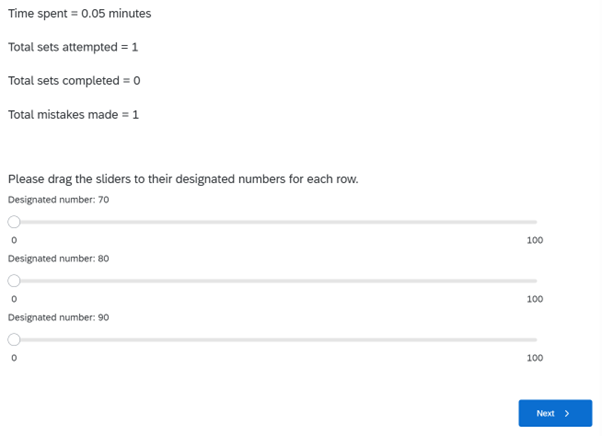
\includegraphics[width=0.75\linewidth]{survey_screenshots/slider_task_set_example.png}
\caption{Example of a set in the slider task}\label{fig:slider-set-example}
\end{figure}

The task is tedious, so effort is costly, and simple, so performance depends more on effort than on skill or education. Its abstractness is deliberate: the aim is to identify how people respond to multiple targets in general rather than in a particular job. Five minutes at low stakes is far from a real job, but it captures how a worker responds to targets within a single task, such as one delivery or one ride.

\subsection{Targets, assessment criteria and action plans}

\paragraph{Targets.} Treated participants were told that they were ``expected to achieve both'' of two targets: complete at least 45 sets, and have at most 10\% of attempted sets \emph{recorded} as mistakes. The targets carried no financial consequences. They were induced as reference points by psychological priming: the instructions presented them as expectations and told participants that others ``generally find achieving both targets manageable under a lenient criterion but highly challenging under a strict criterion''. This follows the idea that goals act as reference points \parencite{heath.1999.goalsreference}. The targets were calibrated on a small trial run with acquaintances who were asked to work as fast and as accurately as they could: no one in the trial met both targets under the strict criterion, and half did under the lenient one.

\paragraph{Assessment criteria (main treatment).} After the task, each treated participant's accuracy was assessed by one of two criteria, drawn at random: a \emph{strict} criterion that records every mistake, or a \emph{lenient} criterion that records only one in four. During the task participants saw their actual mistakes, not their recorded ones. The criterion changes how hard the accuracy target is while leaving the speed target unchanged. For example, a participant who completes exactly 45 sets meets the accuracy target with at most 4 mistakes under the strict criterion (at least 41 correct sets), but with up to 18 under the lenient criterion (27 correct sets). Raising the chance of a strict assessment therefore lowers the probability of meeting the accuracy target, and with it the probability of meeting both targets, while holding the speed target fixed. Taking the trial run as a guide to participants' beliefs, a 75\% chance of lenient assessment implies a probability of meeting both targets of about $0.75 \times 0.5 + 0.25 \times 0 \approx 38\%$, while a 75\% chance of strict assessment implies about $0.25 \times 0.5 + 0.75 \times 0 \approx 13\%$.

\paragraph{Action plan (secondary treatment).} The two targets are stated in different units, so pursuing both requires working out how many mistakes are allowed at each level of speed. Some treated participants were given a table that does this for them (Table~\ref{tab:action-plan}): for each number of sets completed, it lists the maximum number of actual mistakes compatible with the accuracy target under each criterion. The table turns two separate targets into a single plan (``if I complete 45 sets, I can afford 4 mistakes if assessed strictly and 18 if assessed leniently''), which integrates both reference points and spares participants the computation. Under the extended model this should strengthen the response to the targets; under the standard model it should make no difference, since it contains nothing that participants could not work out themselves. I treat this as the secondary test because the manipulation is weaker: participants can do the arithmetic themselves, and whether they used the table is hard to verify.

\begin{table}[htbp]
\centering
\begin{tabular}{@{}ccc@{}}
\toprule
 & \multicolumn{2}{c}{Maximum actual mistakes} \\
\cmidrule(l){2-3}
Sets completed & Strict criterion & Lenient criterion \\
\midrule
35 & 3 & 14 \\
40 & 4 & 16 \\
\textbf{45} & \textbf{4} & \textbf{18} \\
50 & 5 & 20 \\
55 & 5 & 22 \\
\bottomrule
\end{tabular}
\caption{The action plan shown to the \LP{} and \SP{} groups. The bold row corresponds to just meeting both targets.}\label{tab:action-plan}
\end{table}

\subsection{Treatment groups}

Table~\ref{tab:treatment-groups} summarises the four groups. ``Lenient'' and ``Strict'' refer to the criterion that is more likely (75\%) to be applied, and ``Plan'' indicates that the action plan was shown. \Ctrl{} participants were given no targets, were told nothing about assessment criteria, and were assessed strictly. Comparing \LP{} with \Ctrl{} tests whether the targets act as reference points at all, which both models require. Comparing \SP{} with \LP{} is the main test, of the probabilistic expectations channel; comparing \LN{} with \LP{} is the secondary test, of the cognitive complexity channel. Treated participants had to pass a comprehension check before starting the task. The instructions and comprehension check are reproduced in Appendix~\ref{app:survey}.

\begin{table}[htbp]
\centering
\begin{tabularx}{\linewidth}{@{}lll>{\raggedright\arraybackslash}Xl@{}}
\toprule
Group & In tables & Targets & Assessment criterion & Action plan \\
\midrule
\Ctrl{} & Treatment 1 & No & Strict for sure & -- \\
\LP{} & Treatment 2 & Yes & 75\% lenient, 25\% strict & Yes \\
\SP{} & Treatment 3 & Yes & 25\% lenient, 75\% strict & Yes \\
\LN{} & Treatment 4 & Yes & 75\% lenient, 25\% strict & No \\
\bottomrule
\end{tabularx}
\caption{Treatment groups. The second column gives the label used in the generated tables and figures.}\label{tab:treatment-groups}
\end{table}

\subsection{Payment}

Participants were paid a flat amount for taking part, not a piece rate per set. Students received a fixed amount of course credit (0.5\% of the grade in the microeconomics class and 1\% in the macroeconomics class), and lab participants a flat fee (\$1 per five minutes, so pay for the fixed-length task did not depend on performance). Three considerations drove this choice. The first is power. With a fixed budget, every dollar spent on piece rates is a dollar not spent recruiting participants. The power analysis implied that up to 179 participants per group were needed,\footnote{This is an upper bound, for a conservative minimum detectable effect of 0.24 standard deviations and equal outcome variances across groups.} the budget covered only about 200 lab participants even at a flat fee, and the comparisons between treated groups, each a variation on the effect of the targets, need larger samples than detecting the effect of the targets itself. The second is fairness in the student samples: course credit that depended on performance would have depended on a randomly drawn assessment criterion. The third is that a piece rate would have tilted the very trade-off the targets act on, since paying per completed set rewards speed and paying per correct set rewards accuracy. The cost of a flat fee is low stakes, which may have weakened responses to the targets, and it may attract more risk-averse participants \parencite{harrison.2009.riskattitudes}.

\subsection{Samples and implementation}

Participants came from three sources: students in \emph{10000 Principles of Microeconomics} and \emph{10200 Principles of Macroeconomics} at the University of Chicago, recruited through their instructors, and members of the public recruited through the labs of the Roman Family Center for Decision Research (RFCDR) at the University of Chicago Booth School of Business. Within each source, participants were randomly assigned to the four groups with equal probability.\footnote{Equal allocation departs slightly from the optimal allocation based on predicted outcome variances (Appendix~\ref{app:sample-size}), but those predictions were extrapolated from a different experiment and the differences were small.} The student samples were added as a cost-free way to increase the sample size. Neither sample is representative of the general population: the students are a highly selected group, and people who sign up for a behavioural research lab may be more educated or more interested in research than average. Because the aim is to identify how people respond to multiple targets rather than to estimate population averages, this matters less than it otherwise would, but I check whether results differ between the lab and student samples. Running the study online sacrificed some control over the task environment, but made it feasible to run the same protocol with students outside class time and with lab participants.

\subsection{Questionnaire}

After the task, participants could complete an optional, unpaid questionnaire. It recorded gender, race, age, household income, education, whether they had studied economics at university, occupation and whether they used a mouse. It asked how many sets and mistakes they had aimed for, whether they had tried to meet the targets and, if not, why. It also measured loss aversion following \textcite{campos-mercade.2024.gustibusdisputes}: participants stated how many correct sets they would complete under seven fixed piece rates, and under seven random piece rates (a high or a low rate with equal probability) with the same expected values, presented in random order.

\section{Model and hypotheses}\label{sec:model}

\subsection{The standard model}

A participant chooses effort in speed, $e_1$, and in accuracy, $e_2$. Effort in speed raises the number of sets completed, $n(e_1)$; effort in accuracy lowers the mistake rate, $q(e_2)$. The targets are $N$ sets and a mistake rate of $Q$. Consider a simplified version of the KR model with deterministic outcomes, reference points equal to the targets, and linear gain--loss utility:
\[
\begin{aligned}
U = {} & p(e_1, e_2) - c(e_1, e_2) \\
& + \mu_1[(n(e_1)-N)\mathbb{I}(n \geq N) + \lambda_1(n(e_1)-N)\mathbb{I}(n<N)] \\
& + \mu_2[(Q-q(e_2))\mathbb{I}(q \leq Q) + \lambda_2(Q-q(e_2))\mathbb{I}(q>Q)]
\end{aligned}
\]
Here $p(\cdot)$ is the payoff from effort, $c(\cdot)$ is the cost of effort, $\mu_k \geq 0$ is the weight on gain--loss utility in dimension $k$, $\lambda_k \geq 1$ is the loss aversion parameter, and $\mathbb{I}(\cdot)$ is an indicator function. The key feature is additive separability: the gain--loss term for speed depends only on $n$ and $N$, and the one for accuracy only on $q$ and $Q$. How strongly the agent responds to the speed target therefore does not depend on how hard the accuracy target is, except through the cost of effort.

\subsection{The extended model}

I allow the reference points to interact by scaling the whole gain--loss component by two factors:
\[
\begin{aligned}
U = {} & p(e_1, e_2) - c(e_1, e_2) \\
& + \mathbb{P}^E \, \theta \, \bigl\{ \mu_1[(n(e_1)-N)\mathbb{I}(n \geq N) + \lambda_1(n(e_1)-N)\mathbb{I}(n<N)] \\
& \qquad\quad + \mu_2[(Q-q(e_2))\mathbb{I}(q \leq Q) + \lambda_2(Q-q(e_2))\mathbb{I}(q>Q)] \bigr\}
\end{aligned}
\]
The first factor, $\mathbb{P}^E \equiv E[\mathbb{P}(\{n \geq N - \varepsilon \} \cap \{q \leq Q + \varepsilon\})]$, is the agent's expected probability of meeting both targets (to within a bandwidth $\varepsilon$). It captures the idea that targets which are unlikely to be met together lose their motivating force, even if each is attainable on its own. Because $\mathbb{P}^E$ depends on the joint distribution of outcomes in both dimensions, it makes gain--loss utility non-separable: making the accuracy target harder lowers the weight on the speed target too. The second factor, $\theta \geq 0$, is decreasing in the cognitive complexity of relating the two targets to each other: an agent who can easily translate them into a single action plan has a higher $\theta$ and responds more strongly to both. When $\mathbb{P}^E \theta = 1$, the extended model reduces to the standard one.

In the experiment, accuracy is assessed strictly with probability $P_s$ and leniently with probability $P_l = 1 - P_s$. Recording only a quarter of mistakes is equivalent to a target of $4Q$ for the actual mistake rate, so utility becomes
\[
\begin{aligned}
U = {} & p(e_1, e_2) - c(e_1, e_2) + \mathbb{P}^E \, \theta \, [\phi_1 + \phi_2], \quad \text{where} \\
\phi_1 = {} & \mu_1[(n(e_1)-N)\mathbb{I}(n \geq N) + \lambda_1(n(e_1)-N)\mathbb{I}(n<N)], \\
\phi_2 = {} & \mu_2 \bigl\{P_s[(Q-q(e_2))\mathbb{I}(q \leq Q) + \lambda_2(Q-q(e_2))\mathbb{I}(q>Q)] \\
& \quad + P_l[(4Q-q(e_2))\mathbb{I}(q \leq 4Q) + \lambda_2(4Q-q(e_2))\mathbb{I}(q>4Q)]\bigr\}.
\end{aligned}
\]

\subsection{Predictions}

Appendix~\ref{app:derivation} derives the first-order conditions; Table~\ref{tab:predictions} summarises the predictions for each comparison, holding the realised assessment criterion fixed.

Both models predict that the targets change behaviour relative to \Ctrl{}. A participant below a target is in the loss domain, where the marginal value of progress towards it is $\lambda_k \mu_k$ rather than $\mu_k$. Since the speed target was well above what participants achieved without targets, while most already met the accuracy target, both models predict a push towards speed, with an ambiguous effect on accuracy.

The models disagree about the treated groups. In the standard model, a higher chance of strict assessment (\SP{}) makes each mistake more likely to be recorded and so raises the marginal value of accuracy: \SP{} participants should be more accurate than \LP{} participants, possibly at some cost in speed. The action plan adds no information, so \LN{} and \LP{} participants should behave alike. In the extended model, \SP{} lowers $\mathbb{P}^E$ and removing the plan (\LN{}) lowers $\theta$. Both scale down the response to \emph{both} targets, so these groups should behave more like \Ctrl{} than \LP{} does, in both dimensions.

\begin{table}[htbp]
\centering
\begin{tabularx}{\linewidth}{@{}>{\raggedright\arraybackslash}p{0.28\linewidth}>{\raggedright\arraybackslash}X>{\raggedright\arraybackslash}X@{}}
\toprule
Comparison & Standard KR model & Extended model \\
\midrule
\LP{} vs \Ctrl{} \newline (do the targets matter?) & More effort towards speed; ambiguous effect on accuracy & Same \\
\addlinespace
\SP{} vs \LP{} \newline (main test) & More accurate; same speed or slower & Weaker response in both dimensions (closer to \Ctrl{}) \\
\addlinespace
\LN{} vs \LP{} \newline (secondary test) & No difference & Weaker response in both dimensions (closer to \Ctrl{}) \\
\bottomrule
\end{tabularx}
\caption{Predictions of the two models}\label{tab:predictions}
\end{table}

\noindent The results section tests these predictions in order:

\begin{itemize}
\item H0 (both models): the targets change behaviour relative to \Ctrl{}, shifting effort towards speed.
\item H1 (main test): \SP{} participants respond less to the targets than \LP{} participants, in both dimensions. The standard model predicts the opposite for accuracy.
\item H2 (secondary test): \LN{} participants respond less to the targets than \LP{} participants. The standard model predicts no difference.
\end{itemize}

\section{Sample and descriptive statistics}

\subsection{Sample and balance}

The sample consists of the \NumObs{} participants who completed the study:\footnote{\NumRespondents{} people started it.} \NumObsLab{} from the RFCDR lab and \NumObsClass{} from the two classes (\NumObsMicro{} in microeconomics and \NumObsMacro{} in macroeconomics). Table~\ref{tab:covariates-sumstats-pooled} describes the pooled sample by group, and Tables~\ref{tab:covariates-sumstats-lab}--\ref{tab:covariates-sumstats-macro} in Appendix~\ref{app:figures-tables} describe each source. As expected of a largely student sample, participants are young (mean age 23), mostly college-educated, and disproportionately Asian and from high-income households. The lab sample differs from the class samples mainly in being older (mean age 30), mostly female, and more evenly spread across income brackets.

Randomisation produced balanced groups. A joint likelihood ratio test does not reject balance across the four groups in the pooled sample ($\chi^2 = \BalancePooledChisq{}$, $p = \BalancePooledPval{}$) or in any of the three sources (the lowest is $p = \BalanceLabPval{}$, in the lab sample). Covariate by covariate, only two tests reject at or near the 5\% level, both in the lab sample (race, $p = 0.050$, and having studied economics, $p = 0.017$), which is about what chance alone would produce across this many tests. Models 2 and 4 of the regressions below control for the covariates.

\begin{table}[htbp]
\centering
{\fontsize{9.0pt}{11.0pt}\selectfont
\begin{tabular*}{\linewidth}{@{\extracolsep{\fill}}>{\raggedright\arraybackslash}p{\dimexpr 131.25pt -2\tabcolsep-1.5\arrayrulewidth}ccccc>{\centering\arraybackslash}p{\dimexpr 37.50pt -2\tabcolsep-1.5\arrayrulewidth}>{\centering\arraybackslash}p{\dimexpr 37.50pt -2\tabcolsep-1.5\arrayrulewidth}}
\toprule
 &  & \multicolumn{4}{c}{\textbf{Treatments}} &  &  \\ 
\cmidrule(lr){3-6}
\textbf{Metric} & \textbf{All}\textsuperscript{\textit{1}} & \textbf{1}\textsuperscript{\textit{1}} & \textbf{2}\textsuperscript{\textit{1}} & \textbf{3}\textsuperscript{\textit{1}} & \textbf{4}\textsuperscript{\textit{1}} & \textbf{p-value}\textsuperscript{\textit{2,3}} & \textbf{p-value}\textsuperscript{\textit{3,4}} \\ 
\midrule\addlinespace[2.5pt]
{\bfseries Gender} &  &  &  &  &  & 0.7 & 0.7 \\ 
    Male & 299 (48\%) & 79 (47\%) & 64 (44\%) & 79 (54\%) & 77 (48\%) &  &  \\ 
    Female & 314 (51\%) & 88 (52\%) & 79 (54\%) & 66 (45\%) & 81 (50\%) &  &  \\ 
    Non-binary & 8 (1.3\%) & 2 (1.2\%) & 2 (1.4\%) & 1 (0.7\%) & 3 (1.9\%) &  &  \\ 
{\bfseries Race} &  &  &  &  &  & 0.3 & 0.3 \\ 
    White & 236 (39\%) & 70 (42\%) & 52 (36\%) & 51 (36\%) & 63 (41\%) &  &  \\ 
    Asian & 237 (39\%) & 55 (33\%) & 67 (46\%) & 56 (39\%) & 59 (38\%) &  &  \\ 
    Black & 52 (8.5\%) & 18 (11\%) & 5 (3.4\%) & 18 (13\%) & 11 (7.1\%) &  &  \\ 
    Hispanic & 59 (9.7\%) & 17 (10\%) & 14 (9.7\%) & 13 (9.1\%) & 15 (9.7\%) &  &  \\ 
    Mixed & 26 (4.3\%) & 7 (4.2\%) & 7 (4.8\%) & 5 (3.5\%) & 7 (4.5\%) &  &  \\ 
{\bfseries Age} & 23 (8) & 23 (9) & 24 (9) & 24 (8) & 23 (6) & 0.3 & 0.5 \\ 
{\bfseries Household Income} &  &  &  &  &  & 0.5 & 0.5 \\ 
    0 - 24,999 & 69 (12\%) & 22 (14\%) & 17 (13\%) & 10 (7.5\%) & 20 (14\%) &  &  \\ 
    25,000 - 49,999 & 47 (8.4\%) & 11 (7.2\%) & 9 (6.9\%) & 13 (9.7\%) & 14 (9.9\%) &  &  \\ 
    50,000 - 74,999 & 51 (9.1\%) & 14 (9.2\%) & 14 (11\%) & 16 (12\%) & 7 (4.9\%) &  &  \\ 
    75,000 - 119,999 & 68 (12\%) & 22 (14\%) & 13 (10\%) & 13 (9.7\%) & 20 (14\%) &  &  \\ 
    120,000 - 199,999 & 77 (14\%) & 20 (13\%) & 22 (17\%) & 20 (15\%) & 15 (11\%) &  &  \\ 
    200,000 and over & 247 (44\%) & 64 (42\%) & 55 (42\%) & 62 (46\%) & 66 (46\%) &  &  \\ 
{\bfseries Education Level} &  &  &  &  &  & 0.6 & 0.6 \\ 
    Below high school diploma & 1 (0.2\%) & 0 (0\%) & 1 (0.7\%) & 0 (0\%) & 0 (0\%) &  &  \\ 
    High school diploma & 41 (6.5\%) & 11 (6.3\%) & 12 (8.2\%) & 7 (4.7\%) & 11 (6.7\%) &  &  \\ 
    College degree or above & 592 (93\%) & 165 (94\%) & 133 (91\%) & 141 (95\%) & 153 (93\%) &  &  \\ 
{\bfseries Studied Economics} & 487 (77\%) & 136 (77\%) & 110 (75\%) & 118 (80\%) & 123 (75\%) & 0.7 & 0.7 \\ 
{\bfseries Occupation} &  &  &  &  &  & 0.7 & 0.6 \\ 
    Student & 501 (80\%) & 140 (80\%) & 120 (82\%) & 111 (77\%) & 130 (79\%) &  &  \\ 
    Academia & 30 (4.8\%) & 6 (3.4\%) & 6 (4.1\%) & 6 (4.1\%) & 12 (7.3\%) &  &  \\ 
    Clerical & 13 (2.1\%) & 2 (1.1\%) & 4 (2.7\%) & 6 (4.1\%) & 1 (0.6\%) &  &  \\ 
    High-tech mfg or eng & 11 (1.7\%) & 2 (1.1\%) & 1 (0.7\%) & 2 (1.4\%) & 6 (3.7\%) &  &  \\ 
    Managerial & 13 (2.1\%) & 4 (2.3\%) & 3 (2.0\%) & 3 (2.1\%) & 3 (1.8\%) &  &  \\ 
    Professional services & 45 (7.1\%) & 13 (7.5\%) & 9 (6.1\%) & 13 (9.0\%) & 10 (6.1\%) &  &  \\ 
    Unemployed & 11 (1.7\%) & 4 (2.3\%) & 2 (1.4\%) & 3 (2.1\%) & 2 (1.2\%) &  &  \\ 
    Other & 6 (1.0\%) & 3 (1.7\%) & 2 (1.4\%) & 1 (0.7\%) & 0 (0\%) &  &  \\ 
{\bfseries Used Mouse} & 252 (40\%) & 68 (38\%) & 60 (42\%) & 61 (42\%) & 63 (39\%) & 0.9 & 0.9 \\ 
\bottomrule
\end{tabular*}
\begin{minipage}{\linewidth}
\textsuperscript{\textit{1}}n (\%); Mean (SD)\\
\textsuperscript{\textit{2}}Fisher's Exact Test for Count Data with simulated p-value
(based on 10000 replicates); Kruskal-Wallis rank sum test\\
\textsuperscript{\textit{3}}*p\textless{}0.05; **p\textless{}0.01; ***p\textless{}0.001\\
\textsuperscript{\textit{4}}Pearson's Chi-squared test; One-way analysis of means (not assuming equal variances)\\
\end{minipage}
\par}
\caption{Covariates by treatment group (pooled sample). \TreatmentKey}\label{tab:covariates-sumstats-pooled}
\end{table}

\subsection{Performance by sample}

Students completed more sets than lab participants (about 26 against 22.4 on average; $p < 0.001$ for each class against the lab, Welch $t$-tests), although they were less likely to use a mouse (31--32\% against 58\%). Mistake rates are about 7\% in all three sources (Table~\ref{tab:slider-performance-sumstats}). The two class samples do not differ from each other in any measure, so I combine them into one class sample and report results for the pooled sample and, as a robustness check, for the lab and class samples separately. All regressions control for baseline speed in the demo task, which absorbs much of the difference between sources.

\subsection{The speed--accuracy trade-off}

The design relies on speed and accuracy being in tension. Figure~\ref{fig:effort-tradeoffs-1} plots each participant's mistake rate against sets completed, with a local regression (loess) fit. Most participants completed 15--35 sets with low mistake rates, and nearly half (48\%) made no mistakes at all. The fitted curve is flat over this range and rises steeply above about 30 sets, where a handful of participants completed many sets with most or all of them wrong; it also rises at the far left, where a few participants completed few sets and made many mistakes. A reading consistent with this shape is that most participants held accuracy roughly fixed and varied speed, that the trade-off bound only for the few who gave up accuracy for speed, and that the few at the bottom left exerted little effort in either dimension. Because both ends of the curve rest on few observations, this reading is only suggestive. The figure also compares different participants, so it mixes the trade-off each participant faces with differences in ability: able participants can be both fast and accurate. A flat curve across participants is therefore compatible with a steep trade-off for each of them.

Figure~\ref{fig:effort-tradeoffs-2} drops observations outside Tukey's fences (more than 1.5 times the interquartile range beyond the quartiles), applied separately to sets completed and the mistake rate. This removes 62 participants (10\%), almost all for having a mistake rate above 17.9\%; the rest completed fewer than 9 sets.% Counts computed from data/slider_full_data_clean.rds using the rule in code/descriptive_figures.R
\ The rule is poorly suited to the mistake rate, whose distribution is heavily skewed with almost half its mass at zero: it classifies the whole upper tail as outliers, even though these are genuine choices rather than recording errors, and they are precisely the observations that reveal the trade-off. Panel (b) is therefore best read as a view of the bulk of the distribution rather than as a robustness check. Within that bulk the relationship is close to flat, with at most a slight upward slope.\footnote{The curved bands in panel (b) are mechanical: a fixed number of mistakes produces a mistake rate that falls as more sets are attempted.} No observations are excluded from any other analysis.

\begin{figure}[htbp]
\centering
\begin{subfigure}{\linewidth}
\centering
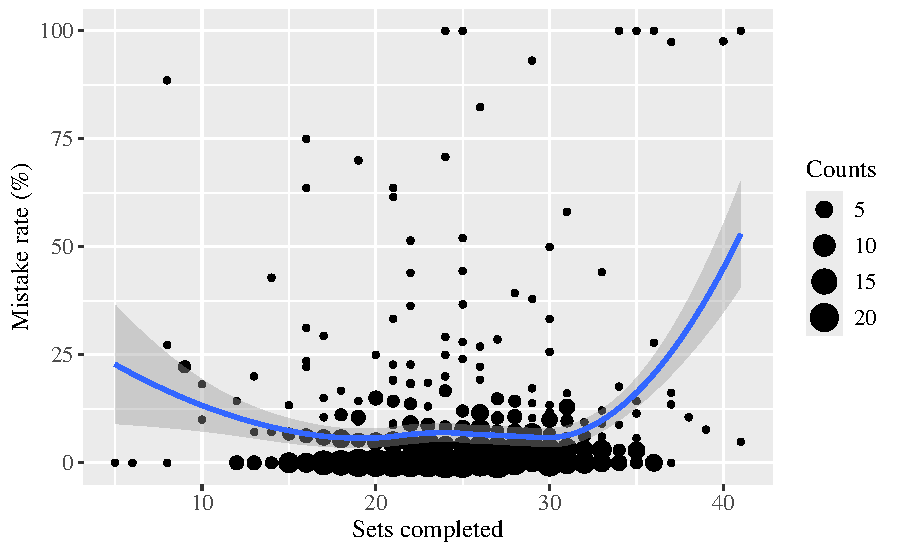
\includegraphics[width=0.75\linewidth]{output/figures/effort_tradeoffs_all.pdf}
\caption{All participants}\label{fig:effort-tradeoffs-1}
\end{subfigure}
\begin{subfigure}{\linewidth}
\centering
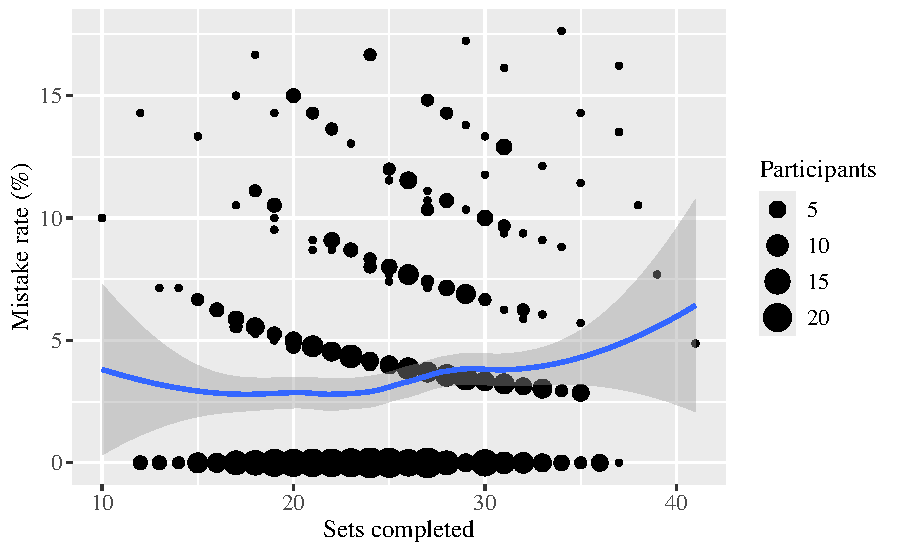
\includegraphics[width=0.75\linewidth]{output/figures/effort_tradeoffs_no_outliers.pdf}
\caption{Excluding participants outside Tukey's fences on either measure (62 of \NumObs{})}\label{fig:effort-tradeoffs-2}
\end{subfigure}
\caption{Speed and accuracy in the slider task. Point size shows the number of participants; the line is a loess fit with its 95\% confidence band.}\label{fig:effort-tradeoffs}
\end{figure}

\section{Results}

\subsection{Empirical strategy}

I compare the groups in two ways. The first is non-parametric: a Kruskal--Wallis test across all four groups and pairwise Kolmogorov--Smirnov tests of the distributions of sets completed and the mistake rate. The second is regression. Because no participant reached the speed target, the main regression is a logit for whether participant $i$ met the accuracy target:
\[
\log \frac{\mathbb{P}(A_i = 1)}{\mathbb{P}(A_i = 0)} = \beta_{1} + \beta_2 T_{2i} +\beta_3 T_{3i} +\beta_4 T_{4i} + \theta\, strict_i + \eta' X_i \tag{1}
\]
where $A_i$ indicates a recorded mistake rate of at most 10\%, $T_{ji}$ indicates membership of group $j$ (numbered as in Table~\ref{tab:treatment-groups}, with \Ctrl{} omitted), $strict_i$ indicates that the strict criterion was applied, and $X_i$ contains covariates and baseline performance in the demo task. Coefficients are changes in the log odds of meeting the accuracy target. Two linear regressions, with heteroskedasticity-robust standard errors, capture changes in effort that need not move participants across the target:
\begin{align*}
mistakerate_i &= \gamma_1 + \gamma_2 T_{2i} + \gamma_3 T_{3i} + \gamma_4 T_{4i} + \phi\, strict_i + \psi' X_i + \varepsilon_i \tag{2} \\
setscompleted_i &= \delta_1 + \delta_2 T_{2i} + \delta_3 T_{3i} + \delta_4 T_{4i} + \mu\, strict_i + \nu' X_i + \varepsilon_i \tag{3}
\end{align*}
Each regression is estimated with the treatment indicators and $strict_i$ only (Model 1), adding covariates (Model 2), adding baseline performance instead (Model 3), and adding both (Model 4). Models 2 and 4 use the 549 participants who answered all covariate questions. I focus on Models 3 and 4. Baseline performance is measured before treatment and is by far the most informative control: it raises the adjusted $R^2$ of the sets-completed regression from 0.01 to 0.45 (Table~\ref{tab:reg-sets}).\footnote{Standard errors for Model 4 of the mistake-rate regression could not be computed, because the outcome is concentrated at zero relative to the number of regressors.}

H1 and H2 are stated in terms of magnitudes: the extended model predicts $|\beta_3| < |\beta_2|$ and $|\beta_4| < |\beta_2|$, and likewise for $\gamma$ and $\delta$. Magnitudes rather than signs are what matter because the direction of the response depends on where participants start relative to each target, which differs between dimensions. I treat H1 and H2 as separate questions rather than one family of hypotheses, since each stands on its own given H0, and so do not adjust their p-values jointly.

\subsection{Do the targets act as reference points?}

Both tests rest on the premise that the primed targets act as reference points, so I first compare \LP{} with \Ctrl{}. In every group, participants were far from the speed target and close to or beyond the accuracy target (Table~\ref{tab:slider-performance-sumstats}). \Ctrl{} participants completed \ControlMeanSets{} sets on average, about half the target, and no participant in any group reached 45 (the maximum was 41). By contrast, most participants met the accuracy target without being asked to: 83\% of \Ctrl{} participants had a mistake rate of 10\% or less, and about half made no mistakes at all.% Shares computed from data/slider_full_data_clean.rds

The targets moved effort towards speed, modestly. \LP{} participants completed 1.2--1.5 more sets than \Ctrl{} participants (Models 3 and 4 of Table~\ref{tab:reg-sets}; the effect is significant at 5\% in all four models), an increase of 5--6\%, or about a fifth of a standard deviation. There is no detectable effect on accuracy. The estimated effects on the probability of meeting the accuracy target (Table~\ref{tab:reg-target}) and on the mistake rate (Table~\ref{tab:reg-mistakes}) are imprecise and point in opposite directions, the first towards slightly worse accuracy and the second towards slightly better. The distributions of both outcomes in \LP{} and \Ctrl{} are not significantly different (Figure~\ref{fig:slider-performance-distribution-comparison}; Kolmogorov--Smirnov $p = \DistTestPooledSetsCompletedOneVsTwoPval{}$ for sets and $p = \DistTestPooledMistakeRateOneVsTwoPval{}$ for the mistake rate), which is unsurprising for a shift of about one set against a standard deviation of about six. The response is similar in the lab and class samples, though less precisely estimated (Appendix~\ref{app:figures-tables}).

This pattern is what reference dependence predicts given where participants started. All of them were below the speed target, in the loss domain, where loss aversion makes each additional set more valuable; most were already above the accuracy target, in the gain domain, where additional accuracy is worth less. Targets in both dimensions should therefore pull effort towards speed, as observed.

The response is small, however, and the data cannot tell apart several explanations for this, which are not mutually exclusive.
\begin{itemize}
\item \emph{Participants held their own goals, which competed with the primed targets.} In the questionnaire, the median participant in every group, including \Ctrl{}, reported aiming for zero mistakes. Of the treated participants who did not try to meet both targets, 143 of 159 said they pursued the accuracy target only. This fits internal accuracy goals that were stricter than the external target and that the speed target only partly displaced.
\item \emph{Many participants did not adopt the primed targets as reference points at all.} The targets had no consequences, and 33 of the participants who explained why they did not pursue a target said they did not care about it. In that case the small increase in speed may reflect a demand effect, or the instruction to ``try your best'', rather than reference dependence.
\item \emph{The speed target was out of reach}, which under the extended model itself dampens the response. Participants could see their progress during the task, and those who realised that they would not reach 45 sets had little reason to keep responding to the target. ``Too difficult to achieve'' was the most common reason for not pursuing a target (66 participants). The targets did raise participants' stated speed aims (a median of 30--40 sets in the treated groups, against 20 in \Ctrl{}) far more than their output.
\end{itemize}
These self-reports were collected after the task, from the participants who chose to answer, and may partly rationalise behaviour, so they are suggestive only.% Survey counts computed from data/slider_full_data_clean.rds

\begin{table}[htbp]
\centering
\inputscaled{1.25}{output/tables/performance_sumstats_pooled.tex}

\medskip
\inputscaled{1.25}{output/tables/performance_sumstats_lab.tex}

\medskip
\inputscaled{1.25}{output/tables/performance_sumstats_micro.tex}

\medskip
\inputscaled{1.25}{output/tables/performance_sumstats_macro.tex}
\caption{Slider task performance by sample and treatment group. \TreatmentKey}\label{tab:slider-performance-sumstats}
\end{table}

\begin{figure}[htbp]
\centering
\begin{subfigure}{\linewidth}
\centering
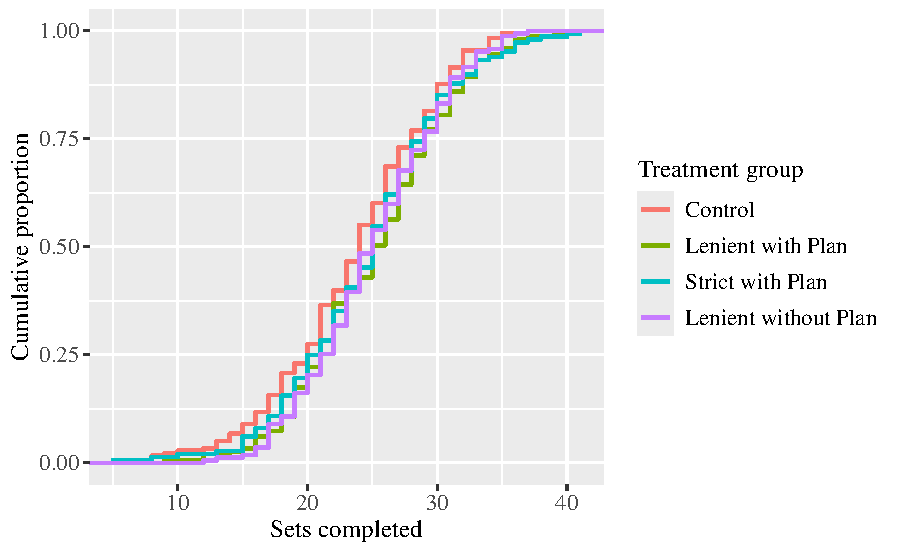
\includegraphics[width=0.75\linewidth]{output/figures/dist_comp_sets_completed_pooled.pdf}
\caption{Sets completed}\label{fig:slider-performance-distribution-comparison-1}
\end{subfigure}
\begin{subfigure}{\linewidth}
\centering
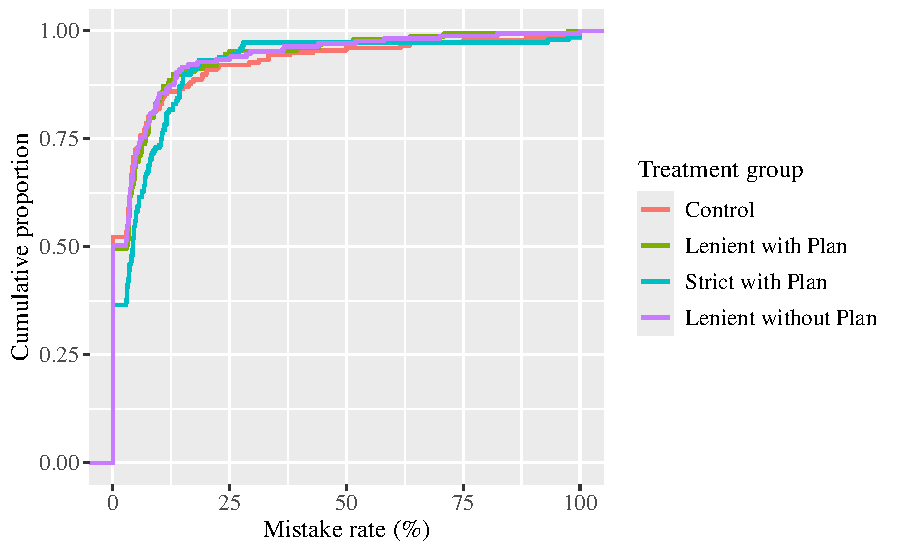
\includegraphics[width=0.75\linewidth]{output/figures/dist_comp_mistake_rate_pooled.pdf}
\caption{Mistake rate}\label{fig:slider-performance-distribution-comparison-2}
\end{subfigure}
\caption{Cumulative distributions of slider task performance by treatment group (pooled sample). \TreatmentKey}\label{fig:slider-performance-distribution-comparison}
\end{figure}

\begin{table}[htbp]
\centering
% Generated by the R scripts in code/; the note is set at the width of the table
\ifdefined\regtablebox\else\newsavebox{\regtablebox}\fi
\sbox{\regtablebox}{%
\begin{tabular}{l c c c c}
\toprule
 & \multicolumn{4}{c}{Log odds of meeting the accuracy target} \\
\cmidrule(lr){2-5}
 & (1) & (2) & (3) & (4) \\
\midrule
Lenient with Plan    & $-0.53$      & $-0.35$      & $-0.76^{*}$  & $-0.54$     \\
                     & $(0.38)$     & $(0.44)$     & $(0.40)$     & $(0.46)$    \\
Strict with Plan     & $-0.52^{*}$  & $-0.57^{*}$  & $-0.42$      & $-0.47$     \\
                     & $(0.29)$     & $(0.33)$     & $(0.32)$     & $(0.37)$    \\
Lenient without Plan & $-0.03$      & $-0.12$      & $-0.08$      & $-0.08$     \\
                     & $(0.43)$     & $(0.47)$     & $(0.46)$     & $(0.51)$    \\
Constant             & $3.41^{***}$ & $3.00^{***}$ & $3.29^{***}$ & $2.36^{**}$ \\
                     & $(0.43)$     & $(0.76)$     & $(0.68)$     & $(0.99)$    \\
\midrule
Baselines            & No           & No           & Yes          & Yes         \\
Covariates           & No           & Yes          & No           & Yes         \\
Observations            & $642$        & $549$        & $642$        & $549$       \\
\bottomrule
\end{tabular}
}%
\begin{minipage}{\wd\regtablebox}
\usebox{\regtablebox}

\smallskip
{\footnotesize\raggedright\textit{Notes:} Logit estimates, with standard errors in parentheses. The outcome is meeting the accuracy target, that is, a recorded mistake rate of at most 10\%. The omitted group is Control. All specifications control for whether the strict criterion was applied. Baselines are sets attempted, sets completed and mistakes in the demo task; covariates are gender, race, household income, education, economics studies, occupation and mouse use. Specifications with covariates use the participants who answered all covariate questions. $^{***}p<0.01$, $^{**}p<0.05$, $^{*}p<0.1$.\par}
\end{minipage}

\caption{Treatment effects on the probability of meeting the accuracy target (pooled sample, logit). \TreatmentKey}\label{tab:reg-target}
\end{table}

\begin{table}[htbp]
\centering
% Generated by the R scripts in code/
\begin{tabular}{l c c c c}
\toprule
 & \multicolumn{4}{c}{Mistake rate (\%)} \\
\cmidrule(lr){2-5}
 & (1) & (2) & (3) & (4) \\
\midrule
Lenient with Plan    & $-2.22$  & $-3.53^{*}$ & $-1.75$  & $-3.56^{**}$ \\
                     & $(1.91)$ & $(1.95)$    & $(1.66)$ & $(1.71)$     \\
Strict with Plan     & $0.30$   & $-0.06$     & $-1.07$  & $-1.62$      \\
                     & $(1.91)$ & $(2.01)$    & $(1.53)$ & $(1.68)$     \\
Lenient without Plan & $-2.37$  & $-2.96$     & $-2.20$  & $-3.06$      \\
                     & $(1.95)$ & $(2.13)$    & $(1.75)$ & $(1.96)$     \\
\midrule
Baselines            & No       & No          & Yes      & Yes          \\
Covariates           & No       & Yes         & No       & Yes          \\
Observations            & $642$    & $547$       & $642$    & $547$        \\
\bottomrule
\end{tabular}

\caption{Treatment effects on the mistake rate (pooled sample). \TreatmentKey}\label{tab:reg-mistakes}
\end{table}

\begin{table}[htbp]
\centering

\begin{tabular}{l c c c c}
\hline
 & \multicolumn{4}{c}{Sets completed} \\
\cline{2-5}
 & Model 1 & Model 2 & Model 3 & Model 4 \\
\hline
(Intercept) & $23.52^{***}$ & $22.60^{***}$ & $8.41^{***}$ & $8.89^{***}$ \\
            & $(0.79)$      & $(1.23)$      & $(0.97)$     & $(1.28)$     \\
treatment2  & $1.69^{*}$    & $1.60^{*}$    & $1.46^{*}$   & $1.24^{*}$   \\
            & $(0.81)$      & $(0.77)$      & $(0.57)$     & $(0.59)$     \\
treatment3  & $1.15$        & $0.74$        & $0.95$       & $0.66$       \\
            & $(0.69)$      & $(0.68)$      & $(0.49)$     & $(0.52)$     \\
treatment4  & $1.53$        & $1.36$        & $1.59^{**}$  & $1.36^{*}$   \\
            & $(0.80)$      & $(0.76)$      & $(0.61)$     & $(0.63)$     \\
\hline
Baselines   & No            & No            & Yes          & Yes          \\
Covariates  & No            & Yes           & No           & Yes          \\
\hline
R$^2$       & $0.01$        & $0.22$        & $0.46$       & $0.53$       \\
Adj. R$^2$  & $0.01$        & $0.18$        & $0.45$       & $0.50$       \\
Num. obs.   & $642$         & $549$         & $642$        & $549$        \\
RMSE        & $5.78$        & $5.30$        & $4.29$       & $4.13$       \\
\hline
\multicolumn{5}{l}{\scriptsize{$^{***}p<0.001$; $^{**}p<0.01$; $^{*}p<0.05$}}
\end{tabular}


\caption{Treatment effects on sets completed (pooled sample). \TreatmentKey}\label{tab:reg-sets}
\end{table}

\subsection{Are the responses driven by loss aversion?}

If the response to the targets comes from reference dependence, it should be stronger for more loss-averse participants. I test this by adding each participant's loss aversion, $\lambda_i$, and its interaction with \LP{} to Models 3 and 4:
\[
\log \frac{\mathbb{P}(A_i = 1)}{\mathbb{P}(A_i = 0)} = \pi_1 + \pi_2 T_{2i} + \pi_3 T_{3i} + \pi_4 T_{4i} + \tau_1 \lambda_i + \tau_2(T_{2i} \times \lambda_i) + \rho\, strict_i + \sigma' X_i \tag{4}
\]
with analogous linear regressions (5) and (6) for the mistake rate and sets completed. If the \LP{} response reflects loss aversion, $\tau_2$ should have the same sign as $\pi_2$; in particular, more loss-averse participants should show a larger increase in sets completed and a larger fall in the probability of meeting the accuracy target. I focus on \LP{} because it is the comparison on which both models agree, and to save degrees of freedom.

Loss aversion is estimated following \textcite{campos-mercade.2024.gustibusdisputes}, who assume KR preferences. Participants stated the number of correct sets they would complete under each of seven fixed piece rates and seven random piece rates; each random piece rate pays a high or a low rate with equal probability and has the same expected value as one of the fixed rates. With an effort cost function $c(e) = \frac{1}{\alpha \omega} e^\omega$, as in the original paper and following \textcite{augenblick.2019.experimenttime}, stated effort satisfies approximately
\[
\begin{aligned}
& \log(e_i) \approx J_i + K_i \log(\bar{w}) - L_i \frac{\Delta w}{\bar w}, \quad \text{where} \\
& J_i = \frac {\log(\alpha_i)}{\omega_i - 1}; \quad K_i = \frac {1}{\omega_i - 1}; \quad L_i = \frac {\lambda_i -1}{4(\omega_i - 1)} = \frac {1}{4} K_i (\lambda_i -1)
\end{aligned}
\]
$\bar w$ is the average piece rate, and $\Delta w = w_h - w_l$ is the spread between the high and low piece rates (zero for fixed rates). I estimate the equation for each participant by OLS and recover $\lambda_i$ from $L_i$ and $K_i$.\footnote{Estimates of $\lambda_i$ were top-coded at 4.33, because the largest $\frac{\Delta w}{\bar w}$ in the survey is 1.2 and the logarithm in the exact equation
  \[
  \log(e_i) = J_i + K_i \log(\bar{w}) + K_i \log\Bigl(1 + 0.25 (1 - \lambda_i) \frac{\Delta w}{\bar w}\Bigr)
  \]
  is otherwise undefined. They were bottom-coded at 0, since negative values would imply utility gains from losses.}

The results do not support the reference-point interpretation (Tables~\ref{tab:reg-target-la}--\ref{tab:reg-sets-la}). The interaction has the opposite sign to the prediction for the accuracy target (positive) and for sets completed (negative, and close to zero), and none of the interaction terms is significant. The test is weak, however. The loss aversion measure comes from unincentivised, hypothetical choices, and almost half of the raw estimates (\LambdaOutOfBounds{} of \LambdaEstimated{}) fall outside the range the method allows, \LambdaBelowBound{} of them below zero. The prediction is also ambiguous if participants hold internal accuracy goals: a loss-averse participant is pulled towards accuracy by those goals and towards speed by the external speed target, so loss aversion can amplify either response. I therefore read this check as failing to confirm, rather than refuting, that the responses come from reference points. It adds to the uncertainty about whether the primed targets became reference points at all, which in turn limits what the next two tests can show. Since none of the treatment differences below is significant, I do not pursue the planned analysis of heterogeneous effects.

\begin{table}[htbp]
\centering
% Generated by the R scripts in code/; the note is set at the width of the table
\ifdefined\regtablebox\else\newsavebox{\regtablebox}\fi
\sbox{\regtablebox}{%
\begin{tabular}{l c c}
\toprule
 & \multicolumn{2}{c}{Log odds of meeting the accuracy target} \\
\cmidrule(lr){2-3}
 & (1) & (2) \\
\midrule
Lenient with Plan                        & $-1.09^{*}$   & $-1.25^{*}$   \\
                                         & $(0.59)$      & $(0.68)$      \\
Strict with Plan                         & $-0.33$       & $-0.39$       \\
                                         & $(0.38)$      & $(0.43)$      \\
Lenient without Plan                     & $-0.37$       & $-0.29$       \\
                                         & $(0.52)$      & $(0.57)$      \\
Strict criterion                         & $-2.35^{***}$ & $-2.61^{***}$ \\
                                         & $(0.52)$      & $(0.59)$      \\
Loss aversion ($\lambda_i$)              & $-0.11$       & $-0.13$       \\
                                         & $(0.10)$      & $(0.12)$      \\
Lenient with Plan $\times$ loss aversion & $0.36$        & $0.42$        \\
                                         & $(0.28)$      & $(0.30)$      \\
Constant                                 & $3.88^{***}$  & $3.12^{**}$   \\
                                         & $(0.84)$      & $(1.21)$      \\
\midrule
Baselines                                & Yes           & Yes           \\
Covariates                               & No            & Yes           \\
Observations                                & $503$         & $460$         \\
\bottomrule
\end{tabular}
}%
\begin{minipage}{\wd\regtablebox}
\usebox{\regtablebox}

\smallskip
{\footnotesize\raggedright\textit{Notes:} Logit estimates, with standard errors in parentheses. The outcome is meeting the accuracy target, that is, a recorded mistake rate of at most 10\%. The omitted group is Control. Loss aversion is the participant's estimated $\lambda_i$, top-coded at 4.33 and bottom-coded at 0. Both specifications control for baseline performance in the demo task (sets attempted, sets completed and mistakes); column (2) also controls for gender, race, household income, education, economics studies, occupation and mouse use. The sample is the participants whose loss aversion could be estimated and, in column (2), who answered all covariate questions. $^{***}p<0.01$, $^{**}p<0.05$, $^{*}p<0.1$.\par}
\end{minipage}

\caption{Treatment effects on the probability of meeting the accuracy target, interacted with loss aversion. \TreatmentKey}\label{tab:reg-target-la}
\end{table}

\begin{table}[htbp]
\centering
% Generated by the R scripts in code/; the note is set at the width of the table
\ifdefined\regtablebox\else\newsavebox{\regtablebox}\fi
\sbox{\regtablebox}{%
\begin{tabular}{l c c}
\toprule
 & \multicolumn{2}{c}{Mistake rate (\%)} \\
\cmidrule(lr){2-3}
 & (1) & (2) \\
\midrule
Lenient with Plan                        & $-2.51$     & $-1.83$     \\
                                         & $(1.95)$    & $(2.02)$    \\
Strict with Plan                         & $-1.11$     & $-1.02$     \\
                                         & $(1.61)$    & $(1.68)$    \\
Lenient without Plan                     & $-1.84$     & $-1.40$     \\
                                         & $(2.00)$    & $(2.17)$    \\
Strict criterion                         & $-2.28^{*}$ & $-1.45$     \\
                                         & $(1.35)$    & $(1.21)$    \\
Loss aversion                            & $-0.00$     & $-0.05$     \\
                                         & $(0.52)$    & $(0.58)$    \\
Lenient with Plan $\times$ Loss aversion & $-0.71$     & $-1.07$     \\
                                         & $(0.76)$    & $(0.82)$    \\
Constant                                 & $6.68^{**}$ & $9.04^{**}$ \\
                                         & $(2.75)$    & $(4.38)$    \\
\midrule
Baselines                                & Yes         & Yes         \\
Covariates                               & No          & Yes         \\
Observations                                & $503$       & $453$       \\
\bottomrule
\end{tabular}
}%
\begin{minipage}{\wd\regtablebox}
\usebox{\regtablebox}

\smallskip
{\footnotesize\raggedright\textit{Notes:} OLS estimates, with heteroskedasticity-robust (HC3) standard errors in parentheses. The omitted group is Control. Loss aversion is the participant's estimated $\lambda_i$, top-coded at 4.33 and bottom-coded at 0. Both specifications control for baseline performance in the demo task (sets attempted, sets completed and mistakes); column (2) also controls for gender, race, household income, education level, economics studies, occupation and mouse use. The sample is the participants whose loss aversion could be estimated and, in column (2), who answered all covariate questions, except the few non-binary participants. $^{***}p<0.01$, $^{**}p<0.05$, $^{*}p<0.1$.\par}
\end{minipage}

\caption{Treatment effects on the mistake rate, interacted with loss aversion. \TreatmentKey}\label{tab:reg-mistakes-la}
\end{table}

\begin{table}[htbp]
\centering
% Generated by the R scripts in code/
\begin{tabular}{l c c}
\toprule
 & \multicolumn{2}{c}{Sets completed} \\
\cmidrule(lr){2-3}
 & (1) & (2) \\
\midrule
Lenient with Plan                        & $1.28$       & $1.00$       \\
                                         & $(0.79)$     & $(0.86)$     \\
Strict with Plan                         & $0.71$       & $0.53$       \\
                                         & $(0.56)$     & $(0.63)$     \\
Lenient without Plan                     & $1.45^{**}$  & $1.38^{*}$   \\
                                         & $(0.71)$     & $(0.72)$     \\
Strict criterion                         & $0.15$       & $0.28$       \\
                                         & $(0.54)$     & $(0.55)$     \\
Loss aversion                            & $0.11$       & $0.06$       \\
                                         & $(0.14)$     & $(0.14)$     \\
Lenient with Plan $\times$ Loss aversion & $-0.05$      & $-0.03$      \\
                                         & $(0.26)$     & $(0.27)$     \\
Constant                                 & $8.21^{***}$ & $8.22^{***}$ \\
                                         & $(1.13)$     & $(1.29)$     \\
\midrule
Baselines                                & Yes          & Yes          \\
Covariates                               & No           & Yes          \\
Observations                                & $503$        & $457$        \\
\bottomrule
\end{tabular}

\caption{Treatment effects on sets completed, interacted with loss aversion. \TreatmentKey}\label{tab:reg-sets-la}
\end{table}

\subsection{Main test: does a lower chance of meeting both targets weaken the response?}

\SP{} participants faced the same targets as \LP{} participants but a 75\% rather than a 25\% chance of strict assessment. The standard model predicts that they should take more care over accuracy; the extended model predicts a weaker response to both targets, that is, behaviour closer to \Ctrl{}.

The point estimates line up with the extended model. In Models 3 and 4, the \SP{} coefficients are smaller in magnitude than the \LP{} coefficients in all three regressions: \SP{} raised sets completed by 0.7--1.0 (not significant), against 1.2--1.5 for \LP{}, and its effects on the accuracy target and the mistake rate are closer to zero. There is no sign of the extra care over accuracy that the standard model predicts. The distributions point the same way, more strongly: \SP{} is the only group whose mistake rates differ from the others (Kruskal--Wallis across groups $p = \DistTestPooledMistakeRateAllTreatmentsPval{}$; pairwise Kolmogorov--Smirnov $p = \DistTestPooledMistakeRateOneVsThreePval{}$ against \Ctrl{}, $p = \DistTestPooledMistakeRateTwoVsThreePval{}$ against \LP{} and $p = \DistTestPooledMistakeRateThreeVsFourPval{}$ against \LN{}). Only 37\% of \SP{} participants made no mistakes, against about half in every other group.% Share computed from data/slider_full_data_clean.rds
\ Taken at face value, participants told that both targets would probably be very hard to meet took less care, not more.

None of this is statistically convincing. The differences between the \SP{} and \LP{} coefficients are not significant in any pooled regression (Models 3 and 4: $p = \CoefTestPooledAccuracyTargetModelThreePval{}$ and $\CoefTestPooledAccuracyTargetModelFourPval{}$ for the accuracy target, $p = \CoefTestPooledSetsCompletedModelThreePval{}$ and $\CoefTestPooledSetsCompletedModelFourPval{}$ for sets completed, and $p = \CoefTestPooledMistakeRateModelThreePval{}$ for the mistake rate in Model 3). The difference in mistake rates shrinks once baseline performance is controlled for, and it comes from the class sample; there is none in the lab sample (Appendix~\ref{app:figures-tables}). The subsamples do not agree with each other either. In the lab sample, \SP{} participants responded significantly less than \LP{} participants in the probability of meeting the accuracy target ($p = \CoefTestLabAccuracyTargetModelThreePval{}$ and $\CoefTestLabAccuracyTargetModelFourPval{}$), but had slightly lower mistake rates, as the standard model predicts; in the class sample, \SP{} responded less in sets and mistake rates but not in the accuracy target. Finally, the \SP{} mistake rates differ from those in \Ctrl{} as well as \LP{}, which attenuation alone would not produce: attenuation moves \SP{} towards \Ctrl{}, not beyond it. Disengagement, that is, giving up on accuracy once the joint target seems out of reach, would produce it, and is in the spirit of the extended model. But sampling noise is an equally plausible explanation, since the macroeconomics class \SP{} group had the highest mean mistake rate (12\%) of any group in any sample.

Two features of the design make attenuation hard to detect even if it exists. First, it is a fraction of a response that is itself only about one set: halving the \LP{} response would mean a difference of about 0.6 sets, against standard errors of 0.5--0.6 on each coefficient, so detecting it reliably would take a sample several times larger. Second, because no one could reach the speed target, the realised chance of meeting both targets was zero in both groups. Participants who discovered this during the task would have converged in their beliefs, shrinking the difference in $\mathbb{P}^E$ that the treatment was designed to create.

\subsection{Secondary test: does an action plan strengthen the response?}

\LN{} participants faced the same targets and assessment probabilities as \LP{} participants but were not shown the action plan. The extended model predicts a weaker response without the plan; the standard model predicts no difference. There is no consistent evidence of a difference. \LN{} raised sets completed by 1.4--1.6, slightly more than \LP{}, and its effect on the mistake rate is similar to that of \LP{}; for both outcomes the two groups' coefficients are within a fraction of a standard error of each other. The only hint of attenuation is in the probability of meeting the accuracy target, where the \LN{} coefficient is close to zero while the \LP{} coefficient is negative, but the gap is of the order of one standard error and sets completed point the other way. The distributions of both outcomes in the two groups are almost identical (Kolmogorov--Smirnov $p = \DistTestPooledSetsCompletedTwoVsFourPval{}$ for sets and $p = \DistTestPooledMistakeRateTwoVsFourPval{}$ for the mistake rate). In the lab and class samples the comparison is imprecise and points in no consistent direction.

The manipulation may simply not have changed how well participants understood the targets. Of the \ExplanationResponses{} participants who were shown the plan and answered the question, \ExplanationNotHelpful{} said it did not make the targets easier or more motivating to achieve. Time spent on the instructions admits two readings. \LN{} participants spent far longer on them (\InstructionsTimeTreatmentFour{} seconds on average, against \InstructionsTimeTreatmentTwo{} for \LP{} and \InstructionsTimeTreatmentThree{} for \SP{}). One reading is that participants with the table skimmed it rather than used it. Another is that participants without it spent the extra time working out the relation between sets and mistakes for themselves, so that both groups ended up with a similar plan. On the second reading the plan saved time rather than changing behaviour, and the cognitive complexity channel remains untested rather than refuted.

\section{Conclusion}

This paper asked whether reference points in different dimensions interact, which existing models rule out by assuming that gain--loss utility is additively separable across dimensions. I proposed an extension of the KR model in which the weight on gain--loss utility depends on the expected probability of meeting all targets jointly (the main channel) and on how easily the targets can be combined into one action plan (the secondary channel), and tested it in a real-effort experiment with a speed target and an accuracy target.

The evidence is inconclusive. The targets raised speed modestly. Making the targets jointly harder to reach weakened the response in both dimensions, as the extended model predicts and contrary to the standard model, but not significantly, and the action plan made no difference. Whether the primed targets acted as reference points at all is itself uncertain: participants seemed to bring strong accuracy goals of their own, and a loss aversion check did not support a reference-point interpretation.

The experiment suggests how a better test could be designed. The targets should be calibrated, with pilots on the actual subject pool, so that each is within reach; meeting them should carry real stakes; and the sample should be sized to detect differences between treated groups, not just the effect of the targets. The clearest lesson is that externally set targets compete with the goals people already hold. How people reconcile their own goals with targets set by others is a question for future work, with direct relevance to how organisations set targets for their employees.

\newpage

\printbibliography[heading=bibintoc, title={References}]

\newpage

\appendix

% Number appendix figures and tables by appendix: Figure A1, Table A1, ...
\counterwithin{figure}{section}
\counterwithin{table}{section}
\renewcommand{\thefigure}{\thesection\arabic{figure}}
\renewcommand{\thetable}{\thesection\arabic{table}}

\section{Figures and tables}\label{app:figures-tables}

In all tables and figures, \TreatmentKey

\begin{table}[p]
\centering
{\fontsize{9.0pt}{11.0pt}\selectfont
\begin{tabular*}{\linewidth}{@{\extracolsep{\fill}}>{\raggedright\arraybackslash}p{\dimexpr 131.25pt -2\tabcolsep-1.5\arrayrulewidth}ccccc>{\centering\arraybackslash}p{\dimexpr 37.50pt -2\tabcolsep-1.5\arrayrulewidth}>{\centering\arraybackslash}p{\dimexpr 37.50pt -2\tabcolsep-1.5\arrayrulewidth}}
\toprule
 &  & \multicolumn{4}{c}{\textbf{Treatments}} &  &  \\ 
\cmidrule(lr){3-6}
\textbf{Metric} & \textbf{All}\textsuperscript{\textit{1}} & \textbf{1}\textsuperscript{\textit{1}} & \textbf{2}\textsuperscript{\textit{1}} & \textbf{3}\textsuperscript{\textit{1}} & \textbf{4}\textsuperscript{\textit{1}} & \textbf{p-value}\textsuperscript{\textit{2,3}} & \textbf{p-value}\textsuperscript{\textit{3,4}} \\ 
\midrule\addlinespace[2.5pt]
{\bfseries Gender} &  &  &  &  &  & >0.9 & >0.9 \\ 
    Male & 63 (30\%) & 17 (29\%) & 14 (29\%) & 16 (31\%) & 16 (32\%) &  &  \\ 
    Female & 140 (67\%) & 40 (69\%) & 32 (67\%) & 35 (67\%) & 33 (66\%) &  &  \\ 
    Non-binary & 5 (2.4\%) & 1 (1.7\%) & 2 (4.2\%) & 1 (1.9\%) & 1 (2.0\%) &  &  \\ 
{\bfseries Race} &  &  &  &  &  & 0.050 & 0.14 \\ 
    White & 92 (45\%) & 25 (43\%) & 25 (52\%) & 21 (40\%) & 21 (44\%) &  &  \\ 
    Asian & 68 (33\%) & 13 (22\%) & 18 (38\%) & 18 (35\%) & 19 (40\%) &  &  \\ 
    Black & 24 (12\%) & 10 (17\%) & 0 (0\%) & 9 (17\%) & 5 (10\%) &  &  \\ 
    Hispanic & 16 (7.8\%) & 7 (12\%) & 3 (6.3\%) & 3 (5.8\%) & 3 (6.3\%) &  &  \\ 
    Mixed & 6 (2.9\%) & 3 (5.2\%) & 2 (4.2\%) & 1 (1.9\%) & 0 (0\%) &  &  \\ 
{\bfseries Age} & 30 (11) & 30 (12) & 31 (13) & 30 (11) & 28 (8) & 0.8 & 0.6 \\ 
{\bfseries Household Income} &  &  &  &  &  & 0.7 & 0.7 \\ 
    0 - 24,999 & 46 (23\%) & 12 (22\%) & 12 (27\%) & 8 (16\%) & 14 (29\%) &  &  \\ 
    25,000 - 49,999 & 34 (17\%) & 11 (20\%) & 4 (9.1\%) & 9 (18\%) & 10 (21\%) &  &  \\ 
    50,000 - 74,999 & 34 (17\%) & 9 (16\%) & 9 (20\%) & 11 (22\%) & 5 (10\%) &  &  \\ 
    75,000 - 119,999 & 32 (16\%) & 9 (16\%) & 5 (11\%) & 10 (20\%) & 8 (17\%) &  &  \\ 
    120,000 - 199,999 & 28 (14\%) & 6 (11\%) & 10 (23\%) & 7 (14\%) & 5 (10\%) &  &  \\ 
    200,000 and over & 22 (11\%) & 8 (15\%) & 4 (9.1\%) & 4 (8.2\%) & 6 (13\%) &  &  \\ 
{\bfseries Education Level} &  &  &  &  &  & 0.4 & 0.4 \\ 
    Below high school diploma & 1 (0.5\%) & 0 (0\%) & 1 (2.2\%) & 0 (0\%) & 0 (0\%) &  &  \\ 
    High school diploma & 41 (20\%) & 11 (19\%) & 12 (26\%) & 7 (13\%) & 11 (22\%) &  &  \\ 
    College degree or above & 163 (80\%) & 47 (81\%) & 33 (72\%) & 45 (87\%) & 38 (78\%) &  &  \\ 
{\bfseries Studied Economics} & 58 (28\%) & 18 (31\%) & 10 (21\%) & 22 (42\%) & 8 (16\%) & 0.017* & 0.017* \\ 
{\bfseries Occupation} &  &  &  &  &  & 0.6 & 0.5 \\ 
    Student & 72 (36\%) & 22 (39\%) & 20 (43\%) & 15 (31\%) & 15 (31\%) &  &  \\ 
    Academia & 30 (15\%) & 6 (11\%) & 6 (13\%) & 6 (12\%) & 12 (24\%) &  &  \\ 
    Clerical & 13 (6.5\%) & 2 (3.6\%) & 4 (8.5\%) & 6 (12\%) & 1 (2.0\%) &  &  \\ 
    High-tech mfg or eng & 11 (5.5\%) & 2 (3.6\%) & 1 (2.1\%) & 2 (4.1\%) & 6 (12\%) &  &  \\ 
    Managerial & 13 (6.5\%) & 4 (7.1\%) & 3 (6.4\%) & 3 (6.1\%) & 3 (6.1\%) &  &  \\ 
    Professional services & 45 (22\%) & 13 (23\%) & 9 (19\%) & 13 (27\%) & 10 (20\%) &  &  \\ 
    Unemployed & 11 (5.5\%) & 4 (7.1\%) & 2 (4.3\%) & 3 (6.1\%) & 2 (4.1\%) &  &  \\ 
    Other & 6 (3.0\%) & 3 (5.4\%) & 2 (4.3\%) & 1 (2.0\%) & 0 (0\%) &  &  \\ 
{\bfseries Used Mouse} & 122 (58\%) & 33 (55\%) & 31 (63\%) & 31 (60\%) & 27 (54\%) & 0.8 & 0.8 \\ 
\bottomrule
\end{tabular*}
\begin{minipage}{\linewidth}
\textsuperscript{\textit{1}}n (\%); Mean (SD)\\
\textsuperscript{\textit{2}}Fisher's Exact Test for Count Data with simulated p-value
(based on 10000 replicates); Kruskal-Wallis rank sum test\\
\textsuperscript{\textit{3}}*p\textless{}0.05; **p\textless{}0.01; ***p\textless{}0.001\\
\textsuperscript{\textit{4}}Pearson's Chi-squared test; One-way analysis of means (not assuming equal variances)\\
\end{minipage}
\par}
\caption{Covariates by treatment group (lab sample)}\label{tab:covariates-sumstats-lab}
\end{table}

\begin{table}[p]
\centering
{\fontsize{9.0pt}{11.0pt}\selectfont
\begin{tabular*}{\linewidth}{@{\extracolsep{\fill}}>{\raggedright\arraybackslash}p{\dimexpr 131.25pt -2\tabcolsep-1.5\arrayrulewidth}>{\centering\arraybackslash}p{\dimexpr 56.25pt -2\tabcolsep-1.5\arrayrulewidth}>{\centering\arraybackslash}p{\dimexpr 56.25pt -2\tabcolsep-1.5\arrayrulewidth}>{\centering\arraybackslash}p{\dimexpr 56.25pt -2\tabcolsep-1.5\arrayrulewidth}>{\centering\arraybackslash}p{\dimexpr 56.25pt -2\tabcolsep-1.5\arrayrulewidth}>{\centering\arraybackslash}p{\dimexpr 56.25pt -2\tabcolsep-1.5\arrayrulewidth}>{\centering\arraybackslash}p{\dimexpr 37.50pt -2\tabcolsep-1.5\arrayrulewidth}>{\centering\arraybackslash}p{\dimexpr 37.50pt -2\tabcolsep-1.5\arrayrulewidth}}
\toprule
 &  & \multicolumn{4}{c}{\textbf{Treatments}} &  &  \\ 
\cmidrule(lr){3-6}
\textbf{Metric} & \textbf{All}\textsuperscript{\textit{1}} & \textbf{1}\textsuperscript{\textit{1}} & \textbf{2}\textsuperscript{\textit{1}} & \textbf{3}\textsuperscript{\textit{1}} & \textbf{4}\textsuperscript{\textit{1}} & \textbf{p-value}\textsuperscript{\textit{2,3}} & \textbf{p-value}\textsuperscript{\textit{3,4}} \\ 
\midrule\addlinespace[2.5pt]
{\bfseries Gender} &  &  &  &  &  & 0.2 & 0.2 \\ 
    Male & 139 (62\%) & 40 (66\%) & 28 (54\%) & 39 (72\%) & 32 (54\%) &  &  \\ 
    Female & 86 (38\%) & 21 (34\%) & 24 (46\%) & 15 (28\%) & 26 (44\%) &  &  \\ 
    Non-binary & 1 (0.4\%) & 0 (0\%) & 0 (0\%) & 0 (0\%) & 1 (1.7\%) &  &  \\ 
{\bfseries Race} &  &  &  &  &  & >0.9 & >0.9 \\ 
    White & 82 (37\%) & 25 (41\%) & 15 (29\%) & 19 (37\%) & 23 (40\%) &  &  \\ 
    Asian & 92 (41\%) & 23 (38\%) & 26 (50\%) & 21 (40\%) & 22 (38\%) &  &  \\ 
    Black & 15 (6.7\%) & 3 (4.9\%) & 3 (5.8\%) & 4 (7.7\%) & 5 (8.6\%) &  &  \\ 
    Hispanic & 22 (9.9\%) & 7 (11\%) & 5 (9.6\%) & 5 (9.6\%) & 5 (8.6\%) &  &  \\ 
    Mixed & 12 (5.4\%) & 3 (4.9\%) & 3 (5.8\%) & 3 (5.8\%) & 3 (5.2\%) &  &  \\ 
{\bfseries Age} & 19.89 (1.15) & 19.93 (1.53) & 20.00 (1.13) & 19.88 (0.85) & 19.76 (0.92) & 0.7 & 0.7 \\ 
{\bfseries Household Income} &  &  &  &  &  & 0.6 & 0.7 \\ 
    0 - 24,999 & 12 (6.1\%) & 5 (8.9\%) & 3 (6.7\%) & 1 (2.1\%) & 3 (6.1\%) &  &  \\ 
    25,000 - 49,999 & 9 (4.6\%) & 0 (0\%) & 4 (8.9\%) & 3 (6.4\%) & 2 (4.1\%) &  &  \\ 
    50,000 - 74,999 & 10 (5.1\%) & 3 (5.4\%) & 2 (4.4\%) & 3 (6.4\%) & 2 (4.1\%) &  &  \\ 
    75,000 - 119,999 & 21 (11\%) & 7 (13\%) & 4 (8.9\%) & 2 (4.3\%) & 8 (16\%) &  &  \\ 
    120,000 - 199,999 & 26 (13\%) & 9 (16\%) & 4 (8.9\%) & 7 (15\%) & 6 (12\%) &  &  \\ 
    200,000 and over & 119 (60\%) & 32 (57\%) & 28 (62\%) & 31 (66\%) & 28 (57\%) &  &  \\ 
{\bfseries Used Mouse} & 71 (31\%) & 19 (30\%) & 15 (28\%) & 19 (37\%) & 18 (30\%) & 0.8 & 0.8 \\ 
\bottomrule
\end{tabular*}
\begin{minipage}{\linewidth}
\textsuperscript{\textit{1}}n (\%); Mean (SD)\\
\textsuperscript{\textit{2}}Fisher's Exact Test for Count Data with simulated p-value
(based on 10000 replicates); Kruskal-Wallis rank sum test\\
\textsuperscript{\textit{3}}*p\textless{}0.05; **p\textless{}0.01; ***p\textless{}0.001\\
\textsuperscript{\textit{4}}Pearson's Chi-squared test; One-way analysis of means (not assuming equal variances)\\
\end{minipage}
\par}
\caption{Covariates by treatment group (microeconomics class sample)}\label{tab:covariates-sumstats-micro}
\end{table}

\begin{table}[p]
\centering
{\fontsize{9.0pt}{11.0pt}\selectfont
\begin{tabular*}{\linewidth}{@{\extracolsep{\fill}}>{\raggedright\arraybackslash}p{\dimexpr 131.25pt -2\tabcolsep-1.5\arrayrulewidth}>{\centering\arraybackslash}p{\dimexpr 56.25pt -2\tabcolsep-1.5\arrayrulewidth}>{\centering\arraybackslash}p{\dimexpr 56.25pt -2\tabcolsep-1.5\arrayrulewidth}>{\centering\arraybackslash}p{\dimexpr 56.25pt -2\tabcolsep-1.5\arrayrulewidth}>{\centering\arraybackslash}p{\dimexpr 56.25pt -2\tabcolsep-1.5\arrayrulewidth}>{\centering\arraybackslash}p{\dimexpr 56.25pt -2\tabcolsep-1.5\arrayrulewidth}>{\centering\arraybackslash}p{\dimexpr 37.50pt -2\tabcolsep-1.5\arrayrulewidth}>{\centering\arraybackslash}p{\dimexpr 37.50pt -2\tabcolsep-1.5\arrayrulewidth}}
\toprule
 &  & \multicolumn{4}{c}{\textbf{Treatments}} &  &  \\ 
\cmidrule(lr){3-6}
\textbf{Metric} & \textbf{All}\textsuperscript{\textit{1}} & \textbf{1}\textsuperscript{\textit{1}} & \textbf{2}\textsuperscript{\textit{1}} & \textbf{3}\textsuperscript{\textit{1}} & \textbf{4}\textsuperscript{\textit{1}} & \textbf{p-value}\textsuperscript{\textit{2,3}} & \textbf{p-value}\textsuperscript{\textit{3,4}} \\ 
\midrule\addlinespace[2.5pt]
{\bfseries Gender} &  &  &  &  &  & 0.6 & 0.6 \\ 
    Male & 97 (52\%) & 22 (44\%) & 22 (49\%) & 24 (60\%) & 29 (56\%) &  &  \\ 
    Female & 88 (47\%) & 27 (54\%) & 23 (51\%) & 16 (40\%) & 22 (42\%) &  &  \\ 
    Non-binary & 2 (1.1\%) & 1 (2.0\%) & 0 (0\%) & 0 (0\%) & 1 (1.9\%) &  &  \\ 
{\bfseries Race} &  &  &  &  &  & 0.4 & 0.4 \\ 
    White & 62 (34\%) & 20 (42\%) & 12 (27\%) & 11 (28\%) & 19 (39\%) &  &  \\ 
    Asian & 77 (43\%) & 19 (40\%) & 23 (51\%) & 17 (44\%) & 18 (37\%) &  &  \\ 
    Black & 13 (7.2\%) & 5 (10\%) & 2 (4.4\%) & 5 (13\%) & 1 (2.0\%) &  &  \\ 
    Hispanic & 21 (12\%) & 3 (6.3\%) & 6 (13\%) & 5 (13\%) & 7 (14\%) &  &  \\ 
    Mixed & 8 (4.4\%) & 1 (2.1\%) & 2 (4.4\%) & 1 (2.6\%) & 4 (8.2\%) &  &  \\ 
{\bfseries Age} & 20.13 (2.00) & 19.72 (2.88) & 20.24 (1.12) & 20.49 (2.27) & 20.13 (1.08) & 0.9 & 0.6 \\ 
{\bfseries Household Income} &  &  &  &  &  & 0.5 & 0.5 \\ 
    0 - 24,999 & 11 (6.6\%) & 5 (12\%) & 2 (4.9\%) & 1 (2.6\%) & 3 (6.7\%) &  &  \\ 
    25,000 - 49,999 & 4 (2.4\%) & 0 (0\%) & 1 (2.4\%) & 1 (2.6\%) & 2 (4.4\%) &  &  \\ 
    50,000 - 74,999 & 7 (4.2\%) & 2 (4.8\%) & 3 (7.3\%) & 2 (5.3\%) & 0 (0\%) &  &  \\ 
    75,000 - 119,999 & 15 (9.0\%) & 6 (14\%) & 4 (9.8\%) & 1 (2.6\%) & 4 (8.9\%) &  &  \\ 
    120,000 - 199,999 & 23 (14\%) & 5 (12\%) & 8 (20\%) & 6 (16\%) & 4 (8.9\%) &  &  \\ 
    200,000 and over & 106 (64\%) & 24 (57\%) & 23 (56\%) & 27 (71\%) & 32 (71\%) &  &  \\ 
{\bfseries Used Mouse} & 59 (32\%) & 16 (30\%) & 14 (33\%) & 11 (28\%) & 18 (35\%) & 0.9 & 0.9 \\ 
\bottomrule
\end{tabular*}
\begin{minipage}{\linewidth}
\textsuperscript{\textit{1}}n (\%); Mean (SD)\\
\textsuperscript{\textit{2}}Fisher's Exact Test for Count Data with simulated p-value
(based on 10000 replicates); Kruskal-Wallis rank sum test\\
\textsuperscript{\textit{3}}*p\textless{}0.05; **p\textless{}0.01; ***p\textless{}0.001\\
\textsuperscript{\textit{4}}Pearson's Chi-squared test; One-way analysis of means (not assuming equal variances)\\
\end{minipage}
\par}
\caption{Covariates by treatment group (macroeconomics class sample)}\label{tab:covariates-sumstats-macro}
\end{table}

\begin{figure}[H]
\centering
\begin{subfigure}{\linewidth}
\centering
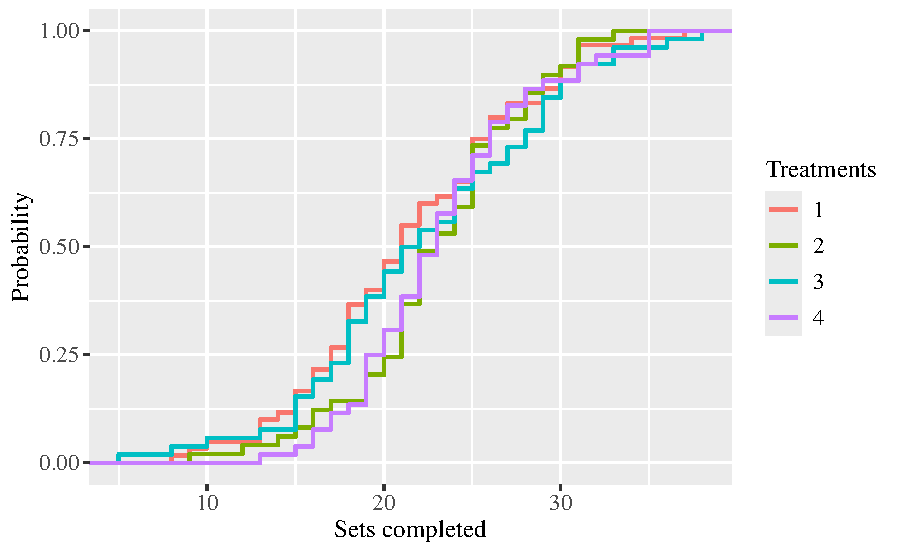
\includegraphics[width=0.75\linewidth]{output/figures/dist_comp_sets_completed_lab.pdf}
\caption{Sets completed}\label{fig:slider-performance-distribution-comparison-lab-1}
\end{subfigure}
\begin{subfigure}{\linewidth}
\centering
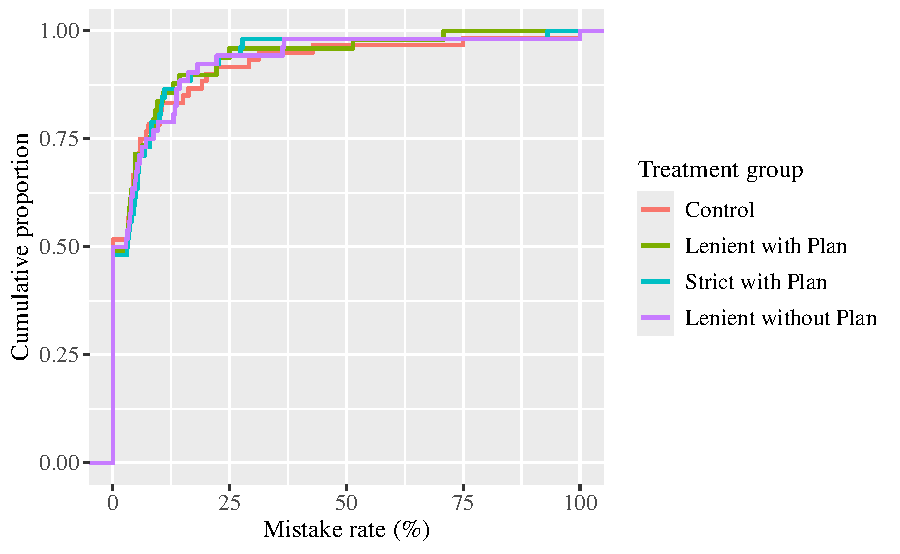
\includegraphics[width=0.75\linewidth]{output/figures/dist_comp_mistake_rate_lab.pdf}
\caption{Mistake rate}\label{fig:slider-performance-distribution-comparison-lab-2}
\end{subfigure}
\caption{Distributions of key performance metrics in the slider task across treatments (lab sample)}\label{fig:slider-performance-distribution-comparison-lab}
\end{figure}

\begin{figure}[htbp]
\centering
\begin{subfigure}{\linewidth}
\centering
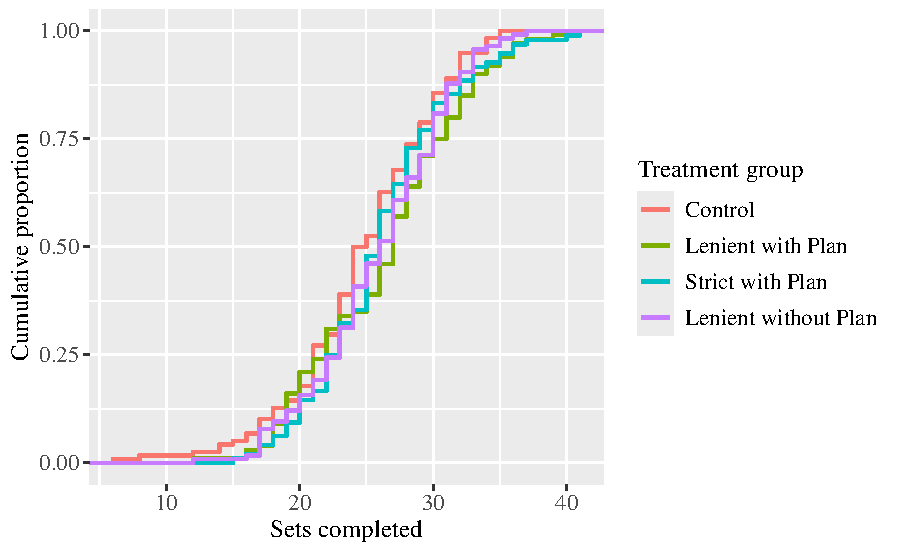
\includegraphics[width=0.75\linewidth]{output/figures/dist_comp_sets_completed_class.pdf}
\caption{Sets completed}\label{fig:slider-performance-distribution-comparison-class-1}
\end{subfigure}
\begin{subfigure}{\linewidth}
\centering
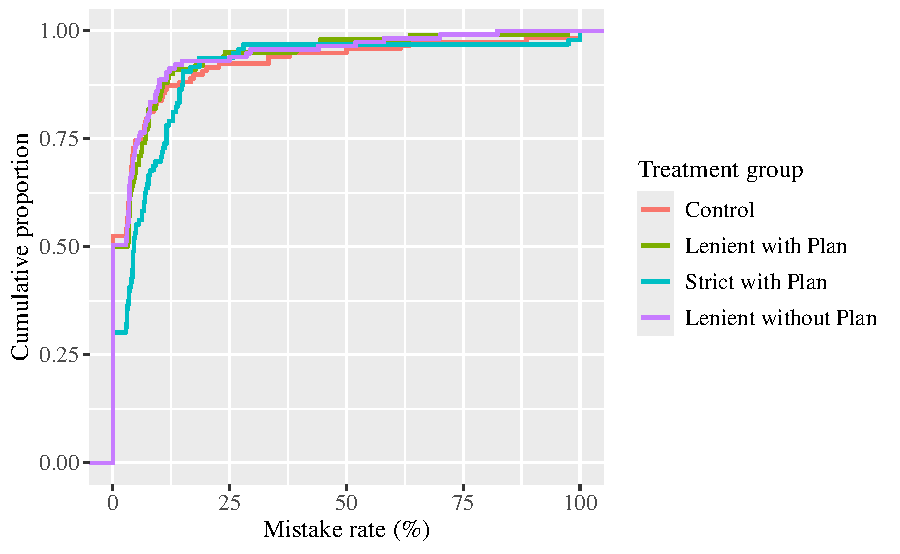
\includegraphics[width=0.75\linewidth]{output/figures/dist_comp_mistake_rate_class.pdf}
\caption{Mistake rate}\label{fig:slider-performance-distribution-comparison-class-2}
\end{subfigure}
\caption{Distributions of key performance metrics in the slider task across treatments (class sample)}\label{fig:slider-performance-distribution-comparison-class}
\end{figure}

\begin{table}[p]
\centering
{\scriptsize\renewcommand{\arraystretch}{0.85}

\begin{tabular}{l c c c c}
\hline
 & \multicolumn{4}{c}{Log odds of achieving accuracy target} \\
\cline{2-5}
 & Model 1 & Model 2 & Model 3 & Model 4 \\
\hline
(Intercept)                     & $3.41^{***}$  & $3.00^{***}$  & $3.29^{***}$  & $2.36^{*}$    \\
                                & $(0.43)$      & $(0.76)$      & $(0.68)$      & $(0.99)$      \\
treatment2                      & $-0.53$       & $-0.35$       & $-0.76$       & $-0.54$       \\
                                & $(0.38)$      & $(0.44)$      & $(0.40)$      & $(0.46)$      \\
treatment3                      & $-0.52$       & $-0.57$       & $-0.42$       & $-0.47$       \\
                                & $(0.29)$      & $(0.33)$      & $(0.32)$      & $(0.37)$      \\
treatment4                      & $-0.03$       & $-0.12$       & $-0.08$       & $-0.08$       \\
                                & $(0.43)$      & $(0.47)$      & $(0.46)$      & $(0.51)$      \\
criterionstrict                 & $-1.81^{***}$ & $-1.97^{***}$ & $-2.22^{***}$ & $-2.31^{***}$ \\
                                & $(0.38)$      & $(0.44)$      & $(0.42)$      & $(0.48)$      \\
genderFemale                    &               & $0.07$        &               & $0.04$        \\
                                &               & $(0.29)$      &               & $(0.31)$      \\
genderNon-binary                &               & $16.05$       &               & $15.37$       \\
                                &               & $(1329.79)$   &               & $(1341.41)$   \\
raceAsian                       &               & $0.36$        &               & $0.21$        \\
                                &               & $(0.32)$      &               & $(0.34)$      \\
raceBlack                       &               & $0.31$        &               & $0.21$        \\
                                &               & $(0.51)$      &               & $(0.55)$      \\
raceHispanic                    &               & $1.05$        &               & $0.89$        \\
                                &               & $(0.60)$      &               & $(0.62)$      \\
raceMixed                       &               & $-0.50$       &               & $-0.22$       \\
                                &               & $(0.58)$      &               & $(0.72)$      \\
income25,000 - 49,999           &               & $-0.18$       &               & $-0.39$       \\
                                &               & $(0.70)$      &               & $(0.73)$      \\
income50,000 - 74,999           &               & $-0.68$       &               & $-0.59$       \\
                                &               & $(0.65)$      &               & $(0.70)$      \\
income75,000 - 119,999          &               & $-1.09$       &               & $-1.26^{*}$   \\
                                &               & $(0.59)$      &               & $(0.64)$      \\
income120,000 - 199,999         &               & $0.44$        &               & $0.20$        \\
                                &               & $(0.69)$      &               & $(0.73)$      \\
income200,000 and over          &               & $-0.70$       &               & $-0.66$       \\
                                &               & $(0.54)$      &               & $(0.58)$      \\
eduBelow high school diploma    &               & $16.37$       &               & $17.18$       \\
                                &               & $(3956.18)$   &               & $(3956.18)$   \\
eduHigh school diploma          &               & $0.44$        &               & $0.64$        \\
                                &               & $(0.61)$      &               & $(0.67)$      \\
econYes                         &               & $0.78$        &               & $0.89^{*}$    \\
                                &               & $(0.43)$      &               & $(0.46)$      \\
occupationAcademia              &               & $0.21$        &               & $0.27$        \\
                                &               & $(0.74)$      &               & $(0.77)$      \\
occupationClerical              &               & $1.09$        &               & $2.17$        \\
                                &               & $(1.16)$      &               & $(1.58)$      \\
occupationHigh-tech mfg or eng  &               & $-0.55$       &               & $-0.45$       \\
                                &               & $(0.90)$      &               & $(0.93)$      \\
occupationManagerial            &               & $-0.29$       &               & $0.41$        \\
                                &               & $(0.85)$      &               & $(0.91)$      \\
occupationProfessional services &               & $1.57$        &               & $2.19^{*}$    \\
                                &               & $(0.81)$      &               & $(0.89)$      \\
occupationUnemployed            &               & $16.28$       &               & $16.77$       \\
                                &               & $(1117.14)$   &               & $(1059.22)$   \\
occupationOther                 &               & $-1.76$       &               & $-2.16^{*}$   \\
                                &               & $(1.02)$      &               & $(1.06)$      \\
mouseYes                        &               & $0.20$        &               & $-0.01$       \\
                                &               & $(0.29)$      &               & $(0.31)$      \\
demo\_sets\_attempted           &               &               & $0.49^{***}$  & $0.47^{**}$   \\
                                &               &               & $(0.14)$      & $(0.17)$      \\
demo\_sets\_completed           &               &               & $-0.28^{*}$   & $-0.15$       \\
                                &               &               & $(0.13)$      & $(0.15)$      \\
demo\_mistakes                  &               &               & $-0.61^{***}$ & $-0.63^{***}$ \\
                                &               &               & $(0.09)$      & $(0.11)$      \\
\hline
AIC                             & $474.96$      & $420.88$      & $419.62$      & $381.34$      \\
BIC                             & $497.28$      & $537.20$      & $455.34$      & $510.59$      \\
Log Likelihood                  & $-232.48$     & $-183.44$     & $-201.81$     & $-160.67$     \\
Num. obs.                       & $642$         & $549$         & $642$         & $549$         \\
\hline
\multicolumn{5}{l}{\scriptsize{$^{***}p<0.001$; $^{**}p<0.01$; $^{*}p<0.05$}}
\end{tabular}

\par}
\caption{Treatment effects on accuracy target achievement likelihood (pooled sample)}\label{tab:reg-target-full}
\end{table}

\begin{table}[p]
\centering
{\scriptsize\renewcommand{\arraystretch}{0.85}
% Generated by the R scripts in code/
\begin{tabular}{l c c c c}
\toprule
 & \multicolumn{4}{c}{Mistake rate (\%)} \\
\cmidrule(lr){2-5}
 & (1) & (2) & (3) & (4) \\
\midrule
Lenient with Plan        & $-2.22$      & $-3.53^{*}$   & $-1.75$      & $-3.56^{**}$  \\
                         & $(1.91)$     & $(1.95)$      & $(1.66)$     & $(1.71)$      \\
Strict with Plan         & $0.30$       & $-0.06$       & $-1.07$      & $-1.62$       \\
                         & $(1.91)$     & $(2.01)$      & $(1.53)$     & $(1.68)$      \\
Lenient without Plan     & $-2.37$      & $-2.96$       & $-2.20$      & $-3.06$       \\
                         & $(1.95)$     & $(2.13)$      & $(1.75)$     & $(1.96)$      \\
Strict criterion         & $-1.22$      & $-1.93$       & $-1.11$      & $-2.24^{*}$   \\
                         & $(1.45)$     & $(1.45)$      & $(1.27)$     & $(1.28)$      \\
Baseline sets attempted  &              &               & $-3.61$      & $-3.31$       \\
                         &              &               & $(2.40)$     & $(2.45)$      \\
Baseline sets completed  &              &               & $3.20$       & $3.08$        \\
                         &              &               & $(2.42)$     & $(2.46)$      \\
Baseline mistakes        &              &               & $5.64^{***}$ & $5.58^{***}$  \\
                         &              &               & $(1.08)$     & $(1.21)$      \\
Female                   &              & $0.69$        &              & $1.63$        \\
                         &              & $(1.31)$      &              & $(1.28)$      \\
Race                     &              &               &              &               \\
\quad Asian              &              & $-3.09^{**}$  &              & $-2.37^{*}$   \\
                         &              & $(1.48)$      &              & $(1.35)$      \\
\quad Black              &              & $-4.87^{***}$ &              & $-2.96^{*}$   \\
                         &              & $(1.72)$      &              & $(1.51)$      \\
\quad Hispanic           &              & $-4.07^{*}$   &              & $-2.18$       \\
                         &              & $(2.10)$      &              & $(2.04)$      \\
\quad Other              &              & $4.79$        &              & $0.04$        \\
                         &              & $(5.54)$      &              & $(4.26)$      \\
Household income         &              &               &              &               \\
\quad \$25,000--49,999   &              & $-0.25$       &              & $-0.70$       \\
                         &              & $(2.27)$      &              & $(2.21)$      \\
\quad \$50,000--74,999   &              & $3.46$        &              & $1.18$        \\
                         &              & $(3.27)$      &              & $(2.79)$      \\
\quad \$75,000--119,999  &              & $5.57^{*}$    &              & $4.05$        \\
                         &              & $(3.06)$      &              & $(2.55)$      \\
\quad \$120,000--199,999 &              & $-3.28^{*}$   &              & $-3.09^{*}$   \\
                         &              & $(1.81)$      &              & $(1.76)$      \\
\quad \$200,000 and over &              & $1.34$        &              & $-0.86$       \\
                         &              & $(2.14)$      &              & $(2.01)$      \\
No college               &              & $0.23$        &              & $-0.24$       \\
                         &              & $(2.97)$      &              & $(2.79)$      \\
Studied economics        &              & $-1.26$       &              & $-1.44$       \\
                         &              & $(1.70)$      &              & $(1.62)$      \\
Student                  &              & $0.87$        &              & $0.94$        \\
                         &              & $(1.72)$      &              & $(1.76)$      \\
Used mouse               &              & $-2.79^{**}$  &              & $-1.56$       \\
                         &              & $(1.28)$      &              & $(1.16)$      \\
Constant                 & $8.96^{***}$ & $11.68^{***}$ & $7.66^{***}$ & $10.27^{***}$ \\
                         & $(1.98)$     & $(3.25)$      & $(2.73)$     & $(3.61)$      \\
\midrule
Observations                & $642$        & $547$         & $642$        & $547$         \\
\bottomrule
\end{tabular}
\par}
\caption{Treatment effects on mistakes rate (pooled sample)}\label{tab:reg-mistakes-full}
\end{table}

\begin{table}[p]
\centering
{\scriptsize\renewcommand{\arraystretch}{0.85}

\begin{tabular}{l c c c c}
\hline
 & \multicolumn{4}{c}{Sets completed} \\
\cline{2-5}
 & Model 1 & Model 2 & Model 3 & Model 4 \\
\hline
(Intercept)                     & $23.52^{***}$ & $22.60^{***}$ & $8.41^{***}$ & $8.89^{***}$  \\
                                & $(0.79)$      & $(1.23)$      & $(0.97)$     & $(1.28)$      \\
treatment2                      & $1.69^{*}$    & $1.60^{*}$    & $1.46^{*}$   & $1.24^{*}$    \\
                                & $(0.81)$      & $(0.77)$      & $(0.57)$     & $(0.59)$      \\
treatment3                      & $1.15$        & $0.74$        & $0.95$       & $0.66$        \\
                                & $(0.69)$      & $(0.68)$      & $(0.49)$     & $(0.52)$      \\
treatment4                      & $1.53$        & $1.36$        & $1.59^{**}$  & $1.36^{*}$    \\
                                & $(0.80)$      & $(0.76)$      & $(0.61)$     & $(0.63)$      \\
criterionstrict                 & $0.09$        & $0.37$        & $0.16$       & $0.21$        \\
                                & $(0.65)$      & $(0.62)$      & $(0.47)$     & $(0.48)$      \\
genderFemale                    &               & $-2.02^{***}$ &              & $-1.03^{**}$  \\
                                &               & $(0.47)$      &              & $(0.39)$      \\
genderNon-binary                &               & $1.51$        &              & $0.84$        \\
                                &               & $(1.77)$      &              & $(1.48)$      \\
raceAsian                       &               & $1.13^{*}$    &              & $0.57$        \\
                                &               & $(0.53)$      &              & $(0.41)$      \\
raceBlack                       &               & $-3.18^{***}$ &              & $-1.45^{*}$   \\
                                &               & $(0.83)$      &              & $(0.62)$      \\
raceHispanic                    &               & $-0.66$       &              & $0.41$        \\
                                &               & $(0.82)$      &              & $(0.67)$      \\
raceMixed                       &               & $0.10$        &              & $-0.15$       \\
                                &               & $(1.33)$      &              & $(1.34)$      \\
income25,000 - 49,999           &               & $-0.15$       &              & $-0.31$       \\
                                &               & $(0.96)$      &              & $(0.75)$      \\
income50,000 - 74,999           &               & $2.90^{**}$   &              & $1.63^{*}$    \\
                                &               & $(1.00)$      &              & $(0.72)$      \\
income75,000 - 119,999          &               & $2.28^{*}$    &              & $1.06$        \\
                                &               & $(0.93)$      &              & $(0.71)$      \\
income120,000 - 199,999         &               & $2.03^{*}$    &              & $0.84$        \\
                                &               & $(0.92)$      &              & $(0.75)$      \\
income200,000 and over          &               & $2.43^{**}$   &              & $0.94$        \\
                                &               & $(0.79)$      &              & $(0.62)$      \\
eduBelow high school diploma    &               & $-5.58^{***}$ &              & $-2.97^{***}$ \\
                                &               & $(1.03)$      &              & $(0.82)$      \\
eduHigh school diploma          &               & $-0.78$       &              & $-0.31$       \\
                                &               & $(0.92)$      &              & $(0.64)$      \\
econYes                         &               & $-0.03$       &              & $0.37$        \\
                                &               & $(0.74)$      &              & $(0.54)$      \\
occupationAcademia              &               & $-1.98$       &              & $-1.17$       \\
                                &               & $(1.06)$      &              & $(0.74)$      \\
occupationClerical              &               & $-0.90$       &              & $-0.45$       \\
                                &               & $(2.27)$      &              & $(1.22)$      \\
occupationHigh-tech mfg or eng  &               & $-2.07$       &              & $-0.13$       \\
                                &               & $(2.33)$      &              & $(1.74)$      \\
occupationManagerial            &               & $-6.03^{*}$   &              & $-2.38$       \\
                                &               & $(2.48)$      &              & $(1.37)$      \\
occupationProfessional services &               & $-2.85^{**}$  &              & $-1.49^{*}$   \\
                                &               & $(0.95)$      &              & $(0.74)$      \\
occupationUnemployed            &               & $-2.11$       &              & $-0.28$       \\
                                &               & $(1.55)$      &              & $(1.12)$      \\
occupationOther                 &               & $-4.89^{*}$   &              & $-3.34^{*}$   \\
                                &               & $(2.16)$      &              & $(1.39)$      \\
mouseYes                        &               & $1.28^{**}$   &              & $1.00^{**}$   \\
                                &               & $(0.48)$      &              & $(0.38)$      \\
demo\_sets\_attempted           &               &               & $1.54^{***}$ & $1.54^{***}$  \\
                                &               &               & $(0.23)$     & $(0.25)$      \\
demo\_sets\_completed           &               &               & $1.76^{***}$ & $1.52^{***}$  \\
                                &               &               & $(0.21)$     & $(0.23)$      \\
demo\_mistakes                  &               &               & $-0.36^{*}$  & $-0.43^{*}$   \\
                                &               &               & $(0.16)$     & $(0.19)$      \\
\hline
R$^2$                           & $0.01$        & $0.22$        & $0.46$       & $0.53$        \\
Adj. R$^2$                      & $0.01$        & $0.18$        & $0.45$       & $0.50$        \\
Num. obs.                       & $642$         & $549$         & $642$        & $549$         \\
RMSE                            & $5.78$        & $5.30$        & $4.29$       & $4.13$        \\
\hline
\multicolumn{5}{l}{\scriptsize{$^{***}p<0.001$; $^{**}p<0.01$; $^{*}p<0.05$}}
\end{tabular}

\par}
\caption{Treatment effects on sets completed (pooled sample)}\label{tab:reg-sets-full}
\end{table}

\begin{table}[p]
\centering
{\scriptsize\renewcommand{\arraystretch}{0.85}
% Generated by the R scripts in code/
\begin{tabular}{l c c c c}
\toprule
 & \multicolumn{4}{c}{Log odds of meeting the accuracy target} \\
\cmidrule(lr){2-5}
 & (1) & (2) & (3) & (4) \\
\midrule
Lenient with Plan        & $-1.26^{*}$   & $-1.74$       & $-1.44^{*}$   & $-2.20^{*}$   \\
                         & $(0.73)$      & $(1.14)$      & $(0.79)$      & $(1.27)$      \\
Strict with Plan         & $0.09$        & $-0.03$       & $0.30$        & $0.23$        \\
                         & $(0.54)$      & $(0.82)$      & $(0.63)$      & $(1.01)$      \\
Lenient without Plan     & $-0.37$       & $-0.62$       & $-0.31$       & $-0.70$       \\
                         & $(0.71)$      & $(0.92)$      & $(0.73)$      & $(1.04)$      \\
Strict criterion         & $-2.71^{***}$ & $-3.56^{***}$ & $-3.11^{***}$ & $-4.16^{***}$ \\
                         & $(0.77)$      & $(1.10)$      & $(0.79)$      & $(1.19)$      \\
Baseline sets attempted  &               &               & $1.64$        & $0.95^{*}$    \\
                         &               &               & $(1.12)$      & $(0.53)$      \\
Baseline sets completed  &               &               & $-1.56$       & $-0.80$       \\
                         &               &               & $(1.18)$      & $(0.54)$      \\
Baseline mistakes        &               &               & $-0.74^{***}$ & $-0.64^{*}$   \\
                         &               &               & $(0.26)$      & $(0.35)$      \\
Female                   &               & $1.66^{**}$   &               & $2.02^{**}$   \\
                         &               & $(0.77)$      &               & $(0.97)$      \\
Race                     &               &               &               &               \\
\quad Asian              &               & $1.23$        &               & $1.34$        \\
                         &               & $(0.75)$      &               & $(0.95)$      \\
\quad Black              &               & $1.40$        &               & $1.35$        \\
                         &               & $(0.96)$      &               & $(1.08)$      \\
\quad Hispanic           &               & $1.55$        &               & $1.34$        \\
                         &               & $(1.75)$      &               & $(2.11)$      \\
\quad Other              &               & $-1.30$       &               & $-0.91$       \\
                         &               & $(1.55)$      &               & $(1.98)$      \\
Household income         &               &               &               &               \\
\quad \$25,000--49,999   &               & $-1.37$       &               & $-1.46$       \\
                         &               & $(1.12)$      &               & $(1.30)$      \\
\quad \$50,000--74,999   &               & $-1.48$       &               & $-1.62$       \\
                         &               & $(1.29)$      &               & $(1.58)$      \\
\quad \$75,000--119,999  &               & $-1.74$       &               & $-1.81$       \\
                         &               & $(1.25)$      &               & $(1.58)$      \\
\quad \$120,000--199,999 &               & $1.28$        &               & $1.06$        \\
                         &               & $(1.99)$      &               & $(2.02)$      \\
\quad \$200,000 and over &               & $-1.61$       &               & $-2.01$       \\
                         &               & $(1.28)$      &               & $(1.57)$      \\
No college               &               & $0.57$        &               & $0.74$        \\
                         &               & $(0.81)$      &               & $(0.93)$      \\
Studied economics        &               & $1.14$        &               & $1.08$        \\
                         &               & $(0.87)$      &               & $(1.10)$      \\
Student                  &               & $-0.22$       &               & $-0.50$       \\
                         &               & $(0.74)$      &               & $(0.88)$      \\
Used mouse               &               & $0.48$        &               & $0.37$        \\
                         &               & $(0.68)$      &               & $(0.80)$      \\
Constant                 & $4.20^{***}$  & $4.05^{**}$   & $4.49^{***}$  & $4.31^{*}$    \\
                         & $(0.84)$      & $(1.70)$      & $(1.28)$      & $(2.37)$      \\
\midrule
Observations                & $213$         & $189$         & $213$         & $189$         \\
\bottomrule
\end{tabular}
\par}
\caption{Treatment effects on accuracy target achievement likelihood (lab sample)}\label{tab:reg-target-lab}
\end{table}

\begin{table}[p]
\centering
{\scriptsize\renewcommand{\arraystretch}{0.85}
% Generated by the R scripts in code/; the note is set at the width of the table
\ifdefined\regtablebox\else\newsavebox{\regtablebox}\fi
\sbox{\regtablebox}{%
\begin{tabular}{l c c c c}
\toprule
 & \multicolumn{4}{c}{Mistake rate (\%)} \\
\cmidrule(lr){2-5}
 & (1) & (2) & (3) & (4) \\
\midrule
Lenient with Plan                            & $-0.52$     & $-2.59$      & $-0.22$      & $-1.60$     \\
                                             & $(3.33)$    & $(4.11)$     & $(3.04)$     & $(3.67)$    \\
Strict with Plan                             & $-1.05$     & $-0.77$      & $-2.58$      & $-2.32$     \\
                                             & $(3.14)$    & $(3.10)$     & $(2.91)$     & $(3.02)$    \\
Lenient without Plan                         & $0.03$      & $1.66$       & $-0.49$      & $1.84$      \\
                                             & $(3.27)$    & $(3.52)$     & $(2.92)$     & $(3.29)$    \\
Strict criterion                             & $1.03$      & $2.48$       & $0.69$       & $1.64$      \\
                                             & $(2.21)$    & $(2.78)$     & $(1.99)$     & $(2.39)$    \\
Baseline sets attempted                      &             &              & $-10.69$     & $-9.87^{*}$ \\
                                             &             &              & $(7.42)$     & $(5.28)$    \\
Baseline sets completed                      &             &              & $10.25$      & $9.79^{*}$  \\
                                             &             &              & $(7.17)$     & $(5.13)$    \\
Baseline mistakes                            &             &              & $8.27^{***}$ & $8.24^{**}$ \\
                                             &             &              & $(2.90)$     & $(3.40)$    \\
Female                                       &             & $-0.07$      &              & $0.10$      \\
                                             &             & $(1.97)$     &              & $(2.29)$    \\
\textbf{Race}                                &             &              &              &             \\
\quad Asian                                  &             & $-1.44$      &              & $-1.36$     \\
                                             &             & $(2.56)$     &              & $(2.60)$    \\
\quad Black                                  &             & $-7.45^{**}$ &              & $-4.05$     \\
                                             &             & $(3.58)$     &              & $(3.11)$    \\
\quad Hispanic                               &             & $-7.77^{*}$  &              & $-5.32$     \\
                                             &             & $(3.97)$     &              & $(4.13)$    \\
\quad Mixed                                  &             & $14.61$      &              & $10.01$     \\
                                             &             & $(18.92)$    &              & $(11.19)$   \\
\textbf{Household income}                    &             &              &              &             \\
\quad \$25,000--49,999                       &             & $2.86$       &              & $1.89$      \\
                                             &             & $(3.11)$     &              & $(2.93)$    \\
\quad \$50,000--74,999                       &             & $3.94$       &              & $0.90$      \\
                                             &             & $(3.86)$     &              & $(2.76)$    \\
\quad \$75,000--119,999                      &             & $5.97$       &              & $6.58$      \\
                                             &             & $(5.53)$     &              & $(4.22)$    \\
\quad \$120,000--199,999                     &             & $0.05$       &              & $1.70$      \\
                                             &             & $(3.09)$     &              & $(2.75)$    \\
\quad \$200,000 and over                     &             & $5.09$       &              & $3.79$      \\
                                             &             & $(5.31)$     &              & $(4.12)$    \\
No college                                   &             & $1.12$       &              & $1.70$      \\
                                             &             & $(4.02)$     &              & $(2.78)$    \\
Studied economics                            &             & $-2.75$      &              & $-1.11$     \\
                                             &             & $(2.81)$     &              & $(2.74)$    \\
\textbf{Occupation}                          &             &              &              &             \\
\quad Academia                               &             & $-1.40$      &              & $-1.17$     \\
                                             &             & $(2.13)$     &              & $(2.24)$    \\
\quad Clerical                               &             & $6.97$       &              & $3.10$      \\
                                             &             & $(9.51)$     &              & $(4.88)$    \\
\quad High-tech manufacturing or engineering &             & $-2.89$      &              & $-3.78$     \\
                                             &             & $(4.13)$     &              & $(3.49)$    \\
\quad Managerial                             &             & $13.60$      &              & $7.76$      \\
                                             &             & $(10.40)$    &              & $(7.41)$    \\
\quad Professional services                  &             & $-0.38$      &              & $-1.53$     \\
                                             &             & $(2.42)$     &              & $(3.04)$    \\
\quad Unemployed                             &             & $-3.14$      &              & $-1.00$     \\
                                             &             & $(2.43)$     &              & $(3.09)$    \\
\quad Other                                  &             & $14.32$      &              & $17.23$     \\
                                             &             & $(11.17)$    &              & $(11.34)$   \\
Used mouse                                   &             & $-2.03$      &              & $-0.64$     \\
                                             &             & $(2.73)$     &              & $(2.17)$    \\
Constant                                     & $6.92^{**}$ & $5.48$       & $6.74$       & $3.13$      \\
                                             & $(3.17)$    & $(4.74)$     & $(4.71)$     & $(7.52)$    \\
\midrule
Observations                                    & $213$       & $186$        & $213$        & $186$       \\
\bottomrule
\end{tabular}
}%
\begin{minipage}{\wd\regtablebox}
\usebox{\regtablebox}

\smallskip
{\raggedright\textit{Notes:} OLS estimates, with heteroskedasticity-robust (HC3) standard errors in parentheses. Omitted categories: Control, lenient criterion, Male, White, \$0--24,999, College degree or above and Student. Baseline variables are from the demo task. Columns (2) and (4) exclude participants with missing covariates and the few non-binary participants. $^{***}p<0.01$, $^{**}p<0.05$, $^{*}p<0.1$.\par}
\end{minipage}
\par}
\caption{Treatment effects on mistake rate (lab sample)}\label{tab:reg-mistakes-lab}
\end{table}

\begin{table}[p]
\centering
{\scriptsize\renewcommand{\arraystretch}{0.85}

\begin{tabular}{l c c c c}
\hline
 & \multicolumn{4}{c}{Sets completed} \\
\cline{2-5}
 & Model 1 & Model 2 & Model 3 & Model 4 \\
\hline
(Intercept)                     & $21.32^{***}$ & $20.42^{***}$ & $6.22^{***}$ & $4.98$  \\
                                & $(1.51)$      & $(1.93)$      & $(1.49)$     & $$      \\
treatment2                      & $1.60$        & $1.34$        & $1.20$       & $1.20$  \\
                                & $(1.58)$      & $(1.48)$      & $(1.02)$     & $$      \\
treatment3                      & $0.88$        & $0.59$        & $0.53$       & $-0.08$ \\
                                & $(1.27)$      & $(1.26)$      & $(0.86)$     & $$      \\
treatment4                      & $1.88$        & $1.43$        & $1.16$       & $0.57$  \\
                                & $(1.44)$      & $(1.35)$      & $(0.89)$     & $$      \\
criterionstrict                 & $0.11$        & $0.86$        & $0.06$       & $0.59$  \\
                                & $(1.28)$      & $(1.16)$      & $(0.75)$     & $$      \\
genderFemale                    &               & $0.20$        &              & $0.58$  \\
                                &               & $(1.00)$      &              & $$      \\
genderNon-binary                &               & $4.27$        &              & $1.93$  \\
                                &               & $(2.29)$      &              & $$      \\
raceAsian                       &               & $2.26$        &              & $1.46$  \\
                                &               & $(1.18)$      &              & $$      \\
raceBlack                       &               & $-3.84^{**}$  &              & $-1.17$ \\
                                &               & $(1.37)$      &              & $$      \\
raceHispanic                    &               & $0.64$        &              & $0.54$  \\
                                &               & $(1.65)$      &              & $$      \\
raceMixed                       &               & $-0.12$       &              & $0.64$  \\
                                &               & $(2.39)$      &              & $$      \\
income25,000 - 49,999           &               & $-0.88$       &              & $-0.44$ \\
                                &               & $(1.28)$      &              & $$      \\
income50,000 - 74,999           &               & $1.42$        &              & $0.10$  \\
                                &               & $(1.29)$      &              & $$      \\
income75,000 - 119,999          &               & $1.19$        &              & $1.26$  \\
                                &               & $(1.43)$      &              & $$      \\
income120,000 - 199,999         &               & $2.58$        &              & $0.72$  \\
                                &               & $(1.52)$      &              & $$      \\
income200,000 and over          &               & $2.82$        &              & $-0.17$ \\
                                &               & $(1.82)$      &              & $$      \\
eduBelow high school diploma    &               & $-6.41^{***}$ &              & $-2.93$ \\
                                &               & $(1.62)$      &              & $$      \\
eduHigh school diploma          &               & $-0.78$       &              & $-0.08$ \\
                                &               & $(0.95)$      &              & $$      \\
econYes                         &               & $-0.09$       &              & $0.43$  \\
                                &               & $(1.03)$      &              & $$      \\
occupationAcademia              &               & $-1.56$       &              & $-0.50$ \\
                                &               & $(1.25)$      &              & $$      \\
occupationClerical              &               & $-0.16$       &              & $-0.23$ \\
                                &               & $(2.21)$      &              & $$      \\
occupationHigh-tech mfg or eng  &               & $-1.11$       &              & $0.43$  \\
                                &               & $(2.40)$      &              & $$      \\
occupationManagerial            &               & $-5.14^{*}$   &              & $-1.19$ \\
                                &               & $(2.53)$      &              & $$      \\
occupationProfessional services &               & $-2.32^{*}$   &              & $-0.76$ \\
                                &               & $(1.13)$      &              & $$      \\
occupationUnemployed            &               & $-1.88$       &              & $-0.11$ \\
                                &               & $(1.73)$      &              & $$      \\
occupationOther                 &               & $-2.87$       &              & $-1.78$ \\
                                &               & $(2.70)$      &              & $$      \\
mouseYes                        &               & $1.41$        &              & $1.33$  \\
                                &               & $(0.84)$      &              & $$      \\
demo\_sets\_attempted           &               &               & $2.27^{**}$  & $2.16$  \\
                                &               &               & $(0.73)$     & $$      \\
demo\_sets\_completed           &               &               & $1.39$       & $1.44$  \\
                                &               &               & $(0.73)$     & $$      \\
demo\_mistakes                  &               &               & $-0.75$      & $-0.54$ \\
                                &               &               & $(0.44)$     & $$      \\
\hline
R$^2$                           & $0.01$        & $0.24$        & $0.57$       & $0.65$  \\
Adj. R$^2$                      & $-0.00$       & $0.12$        & $0.56$       & $0.59$  \\
Num. obs.                       & $213$         & $191$         & $213$        & $191$   \\
RMSE                            & $5.96$        & $5.59$        & $3.95$       & $3.80$  \\
\hline
\multicolumn{5}{l}{\scriptsize{$^{***}p<0.001$; $^{**}p<0.01$; $^{*}p<0.05$}}
\end{tabular}

\par}
\caption{Treatment effects on sets completed (lab sample)}\label{tab:reg-sets-lab}
\end{table}

\begin{table}[p]
\centering
{\scriptsize\renewcommand{\arraystretch}{0.85}
% Generated by the R scripts in code/; the note is set at the width of the table
\ifdefined\regtablebox\else\newsavebox{\regtablebox}\fi
\sbox{\regtablebox}{%
\begin{tabular}{l c c c c}
\toprule
 & \multicolumn{4}{c}{Log odds of meeting the accuracy target} \\
\cmidrule(lr){2-5}
 & (1) & (2) & (3) & (4) \\
\midrule
Lenient with Plan         & $-0.27$       & $-0.17$       & $-0.49$       & $-0.27$       \\
                          & $(0.48)$      & $(0.53)$      & $(0.50)$      & $(0.58)$      \\
Strict with Plan          & $-0.78^{**}$  & $-0.85^{**}$  & $-0.66^{*}$   & $-0.80^{*}$   \\
                          & $(0.35)$      & $(0.41)$      & $(0.40)$      & $(0.47)$      \\
Lenient without Plan      & $0.19$        & $0.09$        & $0.21$        & $0.39$        \\
                          & $(0.51)$      & $(0.53)$      & $(0.63)$      & $(0.69)$      \\
Strict criterion          & $-1.47^{***}$ & $-1.44^{***}$ & $-1.94^{***}$ & $-1.71^{***}$ \\
                          & $(0.42)$      & $(0.44)$      & $(0.52)$      & $(0.54)$      \\
Baseline sets attempted   &               &               & $0.39^{**}$   & $0.32$        \\
                          &               &               & $(0.18)$      & $(0.47)$      \\
Baseline sets completed   &               &               & $-0.11$       & $0.07$        \\
                          &               &               & $(0.16)$      & $(0.43)$      \\
Baseline mistakes         &               &               & $-0.63^{***}$ & $-0.63^{***}$ \\
                          &               &               & $(0.11)$      & $(0.14)$      \\
\textbf{Gender}           &               &               &               &               \\
\quad Female              &               & $-0.11$       &               & $-0.09$       \\
                          &               & $(0.34)$      &               & $(0.40)$      \\
\textbf{Race}             &               &               &               &               \\
\quad Asian               &               & $0.16$        &               & $-0.05$       \\
                          &               & $(0.37)$      &               & $(0.42)$      \\
\quad Black               &               & $-0.38$       &               & $-0.62$       \\
                          &               & $(0.67)$      &               & $(0.68)$      \\
\quad Hispanic            &               & $0.49$        &               & $0.36$        \\
                          &               & $(0.74)$      &               & $(0.86)$      \\
\quad Mixed               &               & $-0.61$       &               & $-0.52$       \\
                          &               & $(0.70)$      &               & $(0.95)$      \\
\textbf{Household income} &               &               &               &               \\
\quad \$25,000--49,999    &               & $15.80^{***}$ &               & $15.51^{***}$ \\
                          &               & $(0.95)$      &               & $(1.08)$      \\
\quad \$50,000--74,999    &               & $0.08$        &               & $0.32$        \\
                          &               & $(1.14)$      &               & $(1.09)$      \\
\quad \$75,000--119,999   &               & $-0.57$       &               & $-0.75$       \\
                          &               & $(0.90)$      &               & $(0.95)$      \\
\quad \$120,000--199,999  &               & $0.69$        &               & $0.56$        \\
                          &               & $(0.94)$      &               & $(0.99)$      \\
\quad \$200,000 and over  &               & $-0.04$       &               & $0.12$        \\
                          &               & $(0.78)$      &               & $(0.86)$      \\
Used mouse                &               & $0.18$        &               & $0.04$        \\
                          &               & $(0.36)$      &               & $(0.42)$      \\
Constant                  & $3.12^{***}$  & $2.96^{***}$  & $2.81^{***}$  & $1.92$        \\
                          & $(0.49)$      & $(0.98)$      & $(0.92)$      & $(1.37)$      \\
\midrule
Observations                 & $429$         & $356$         & $429$         & $356$         \\
\bottomrule
\end{tabular}
}%
\begin{minipage}{\wd\regtablebox}
\usebox{\regtablebox}

\smallskip
{\raggedright\textit{Notes:} Logit estimates, with robust (HC3) standard errors in parentheses. The outcome is meeting the accuracy target, that is, a recorded mistake rate of at most 10\%. Omitted categories: Control, lenient criterion, Male, White and \$0--24,999. Baseline variables are from the demo task. Columns (2) and (4) exclude participants with missing covariates and the few non-binary participants. $^{***}p<0.01$, $^{**}p<0.05$, $^{*}p<0.1$.\par}
\end{minipage}
\par}
\caption{Treatment effects on accuracy target achievement likelihood (class sample)}\label{tab:reg-target-class}
\end{table}

\begin{table}[p]
\centering
{\scriptsize\renewcommand{\arraystretch}{0.85}

\begin{tabular}{l c c c c}
\hline
 & \multicolumn{4}{c}{Mistake rate} \\
\cline{2-5}
 & Model 1 & Model 2 & Model 3 & Model 4 \\
\hline
(Intercept)             & $10.04^{***}$ & $14.05^{***}$ & $7.98^{*}$   & $14.62^{**}$ \\
                        & $(2.52)$      & $(4.19)$      & $(3.65)$     & $(5.49)$     \\
treatment2              & $-2.97$       & $-3.22$       & $-2.72$      & $-3.76$      \\
                        & $(2.34)$      & $(2.30)$      & $(1.94)$     & $(1.96)$     \\
treatment3              & $1.04$        & $0.34$        & $-0.98$      & $-1.05$      \\
                        & $(2.42)$      & $(2.45)$      & $(1.89)$     & $(2.09)$     \\
treatment4              & $-3.67$       & $-3.43$       & $-3.65$      & $-4.18$      \\
                        & $(2.45)$      & $(2.54)$      & $(2.16)$     & $(2.36)$     \\
criterionstrict         & $-2.41$       & $-2.61$       & $-2.16$      & $-3.10^{*}$  \\
                        & $(1.89)$      & $(1.52)$      & $(1.60)$     & $(1.48)$     \\
genderFemale            &               & $1.27$        &              & $1.74$       \\
                        &               & $(1.61)$      &              & $(1.47)$     \\
genderNon-binary        &               & $-5.48$       &              & $-1.77$      \\
                        &               & $(5.00)$      &              & $(4.61)$     \\
raceAsian               &               & $-2.91$       &              & $-2.32$      \\
                        &               & $(1.85)$      &              & $(1.58)$     \\
raceBlack               &               & $-4.36^{*}$   &              & $-2.71$      \\
                        &               & $(2.20)$      &              & $(1.69)$     \\
raceHispanic            &               & $-3.02$       &              & $-1.58$      \\
                        &               & $(2.69)$      &              & $(2.59)$     \\
raceMixed               &               & $-2.60$       &              & $-4.20$      \\
                        &               & $(2.33)$      &              & $(2.41)$     \\
income25,000 - 49,999   &               & $-4.69$       &              & $-3.67$      \\
                        &               & $(3.69)$      &              & $(3.62)$     \\
income50,000 - 74,999   &               & $1.79$        &              & $-0.35$      \\
                        &               & $(6.78)$      &              & $(5.52)$     \\
income75,000 - 119,999  &               & $2.20$        &              & $1.30$       \\
                        &               & $(4.56)$      &              & $(4.16)$     \\
income120,000 - 199,999 &               & $-6.03$       &              & $-6.26$      \\
                        &               & $(3.37)$      &              & $(3.37)$     \\
income200,000 and over  &               & $-1.29$       &              & $-3.26$      \\
                        &               & $(3.43)$      &              & $(3.34)$     \\
mouseYes                &               & $-2.74^{*}$   &              & $-2.36$      \\
                        &               & $(1.31)$      &              & $(1.33)$     \\
demo\_sets\_attempted   &               &               & $-1.71$      & $-0.96$      \\
                        &               &               & $(2.54)$     & $(2.58)$     \\
demo\_sets\_completed   &               &               & $1.45$       & $0.52$       \\
                        &               &               & $(2.58)$     & $(2.62)$     \\
demo\_mistakes          &               &               & $5.07^{***}$ & $4.51^{***}$ \\
                        &               &               & $(1.10)$     & $(1.23)$     \\
\hline
R$^2$                   & $0.01$        & $0.05$        & $0.29$       & $0.28$       \\
Adj. R$^2$              & $-0.00$       & $0.00$        & $0.27$       & $0.24$       \\
Num. obs.               & $429$         & $358$         & $429$        & $358$        \\
RMSE                    & $15.82$       & $15.21$       & $13.48$      & $13.27$      \\
\hline
\multicolumn{5}{l}{\scriptsize{$^{***}p<0.001$; $^{**}p<0.01$; $^{*}p<0.05$}}
\end{tabular}

\par}
\caption{Treatment effects on mistake rates (class sample)}\label{tab:reg-mistakes-class}
\end{table}

\begin{table}[p]
\centering
{\scriptsize\renewcommand{\arraystretch}{0.85}
% Generated by the R scripts in code/; the note is set at the width of the table
\ifdefined\regtablebox\else\newsavebox{\regtablebox}\fi
\sbox{\regtablebox}{%
\begin{tabular}{l c c c c}
\toprule
 & \multicolumn{4}{c}{Sets completed} \\
\cmidrule(lr){2-5}
 & (1) & (2) & (3) & (4) \\
\midrule
Lenient with Plan                & $1.59^{*}$    & $1.55^{*}$    & $1.54^{**}$   & $1.30^{*}$    \\
                                 & $(0.89)$      & $(0.93)$      & $(0.67)$      & $(0.72)$      \\
Strict with Plan                 & $1.34^{*}$    & $0.78$        & $1.22^{**}$   & $0.95$        \\
                                 & $(0.76)$      & $(0.83)$      & $(0.59)$      & $(0.66)$      \\
Lenient without Plan             & $1.13$        & $1.09$        & $1.64^{**}$   & $1.63^{**}$   \\
                                 & $(0.91)$      & $(0.95)$      & $(0.77)$      & $(0.83)$      \\
Strict criterion                 & $-0.07$       & $-0.06$       & $0.15$        & $0.01$        \\
                                 & $(0.71)$      & $(0.73)$      & $(0.57)$      & $(0.60)$      \\
Baseline performance (demo task) &               &               &               &               \\
\quad Sets attempted             &               &               & $1.20^{***}$  & $1.31^{***}$  \\
                                 &               &               & $(0.23)$      & $(0.25)$      \\
\quad Sets completed             &               &               & $1.68^{***}$  & $1.46^{***}$  \\
                                 &               &               & $(0.20)$      & $(0.22)$      \\
\quad Mistakes                   &               &               & $-0.24$       & $-0.39^{*}$   \\
                                 &               &               & $(0.18)$      & $(0.20)$      \\
Gender                           &               &               &               &               \\
\quad Female                     &               & $-2.93^{***}$ &               & $-1.69^{***}$ \\
                                 &               & $(0.53)$      &               & $(0.48)$      \\
\quad Non-binary                 &               & $1.13$        &               & $1.18$        \\
                                 &               & $(4.83)$      &               & $(5.10)$      \\
Race                             &               &               &               &               \\
\quad Asian                      &               & $0.97$        &               & $0.40$        \\
                                 &               & $(0.61)$      &               & $(0.50)$      \\
\quad Black                      &               & $-2.64^{**}$  &               & $-1.43$       \\
                                 &               & $(1.11)$      &               & $(0.91)$      \\
\quad Hispanic                   &               & $-1.33$       &               & $-0.00$       \\
                                 &               & $(0.97)$      &               & $(0.82)$      \\
\quad Mixed                      &               & $-0.12$       &               & $-0.59$       \\
                                 &               & $(1.67)$      &               & $(1.73)$      \\
Household income                 &               &               &               &               \\
\quad \$25,000--49,999           &               & $0.80$        &               & $0.18$        \\
                                 &               & $(1.63)$      &               & $(1.26)$      \\
\quad \$50,000--74,999           &               & $4.59^{***}$  &               & $3.57^{***}$  \\
                                 &               & $(1.57)$      &               & $(1.35)$      \\
\quad \$75,000--119,999          &               & $2.72^{*}$    &               & $0.99$        \\
                                 &               & $(1.41)$      &               & $(1.14)$      \\
\quad \$120,000--199,999         &               & $1.65$        &               & $0.92$        \\
                                 &               & $(1.35)$      &               & $(1.18)$      \\
\quad \$200,000 and over         &               & $2.36^{**}$   &               & $1.20$        \\
                                 &               & $(1.18)$      &               & $(0.95)$      \\
Used mouse                       &               & $1.39^{**}$   &               & $0.93^{*}$    \\
                                 &               & $(0.60)$      &               & $(0.51)$      \\
Constant                         & $24.78^{***}$ & $23.31^{***}$ & $10.84^{***}$ & $10.81^{***}$ \\
                                 & $(0.87)$      & $(1.46)$      & $(1.23)$      & $(1.57)$      \\
\midrule
Observations                        & $429$         & $358$         & $429$         & $358$         \\
\bottomrule
\end{tabular}
}%
\begin{minipage}{\wd\regtablebox}
\usebox{\regtablebox}

\smallskip
{\raggedright\textit{Notes:} OLS estimates, with heteroskedasticity-robust (HC2) standard errors in parentheses. The omitted group is Control. Omitted categories are the lenient criterion and, for covariates, gender (Male), race (White) and household income (\$0--24,999). Specifications with covariates use the participants who answered all covariate questions. $^{***}p<0.01$, $^{**}p<0.05$, $^{*}p<0.1$.\par}
\end{minipage}
\par}
\caption{Treatment effects on sets completed (class sample)}\label{tab:reg-sets-class}
\end{table}

\section{Derivation of first-order conditions for theoretical specification}\label{app:derivation}

Beginning from the utility function,
\[
\begin{aligned}
U = {} & p(e_1, e_2) - c(e_1, e_2) + \mathbb{P}^E \, \theta \, [\phi_1 + \phi_2], \quad \text{where} \\
\phi_1 = {} & \mu_1[(n(e_1)-N)\mathbb{I}(n \geq N) + \lambda_1(n(e_1)-N)\mathbb{I}(n<N)], \\
\phi_2 = {} & \mu_2 \bigl\{P_s[(Q-q(e_2))\mathbb{I}(q \leq Q) + \lambda_2(Q-q(e_2))\mathbb{I}(q>Q)] \\
& \quad + P_l[(4Q-q(e_2))\mathbb{I}(q \leq 4Q) + \lambda_2(4Q-q(e_2))\mathbb{I}(q>4Q)]\bigr\},
\end{aligned}
\]
we can split it into the level component, gain-loss component in the speed dimension, and gain-loss component in the effort dimension, and differentiate each component with respect to effort. First consider the original KR model without $\mathbb{P}^E$ and $\theta$.

The derivative of the level component is uninteresting across treatments as it retains the same functional form as effort exertion and task performance varies.

The matrix of partial derivatives for the gain-loss component in the speed dimension are given by
\[
\begin{aligned}
& n \geq N: [\mu_1 n'(e_1), \: \mu_1 n'(e_1) \frac {de_1}{de_2}] \\
& n < N: [\mu_1 \lambda_1 n'(e_1), \: \mu_1 \lambda_1 n'(e_1) \frac {de_1}{de_2}]
\end{aligned}
\]
Note the discontinuity in the marginal utility of exerting effort at the target N. The agent is more incentivised to exert effort in the speed dimension when below the speed target N than above due to loss aversion as captured by $\lambda>1$. If there are substitution effects between the the two effort dimensions, i.e.~$\frac {de_1}{de_2}<0$, then the inverse will hold true for effort in the accuracy dimension relative to N.

The derivatives for the gain-loss component in the accuracy dimension are given by
\[
\begin{aligned}
& q \leq Q: [\mu_2 |q'(e_2)| \frac {de_2}{de_1}, \: \mu_2 q'(e_2)] \\
& Q < q \leq 4Q: [\mu_2 (P_s \lambda_2 + P_l) |q'(e_2)| \frac {de_2}{de_1}, \: \mu_2 (P_s \lambda_2 + P_l) q'(e_2)] \\
& q > 4Q: [\mu_2 \lambda_2 |q'(e_2)| \frac {de_2}{de_1}, \: \mu_2 \lambda_2 |q'(e_2)|]
\end{aligned}
\]
Similar insights apply for the accuracy dimension, except there are two discontinuities, one corresponding to the achieving the accuracy target under the strict criterion, and the next corresponding to achieving the accuracy target under the lenient criterion. Increasing the probability of getting a strict assessment criteria thus further incentivises agents to strive for the strict accuracy target, leading to a higher probability of achieving the accuracy target holding the assessment criteria constant.

At the optimum,
\[
\begin{aligned}
& c'(e_1, e_2) = p'(e_1, e_2) + \phi_1'(e_1, e_2) + \phi_2'(e_1, e_2) \\
& \frac {MC(e_1)}{MC(e_2)} = \frac {MB(e_1)}{MB(e_2)}
\end{aligned}
\]
Thus, the KR model predicts that when substitution effects between the two effort dimensions are negligible, subjects in \SP{} are more likely to achieve the accuracy target and equally likely to achieve the speed target as compared to \LP{}, or if substitution effects are appreciable, then subjects in \SP{} are more likely to achieve the accuracy target at the expense of the speed target. The KR model does not discriminate effects between \LP{} and \LN{}.

However, when we add the additional parameters, then the first-order conditions become
\[
\begin{aligned}
& c'(e_1, e_2) = p'(e_1, e_2) + \mathbb{P}^E \times \theta \times [\phi_1'(e_1, e_2) + \phi_2'(e_1, e_2)] \\
& \frac {MC(e_1)}{MC(e_2)} = \frac {MB(e_1)}{MB(e_2)}
\end{aligned}
\]
\SP{} lowers $\mathbb{P}^E$ whereas \LN{} lowers $\theta$, thus attenuating the reference point effects and leading to less likely target achievement in either dimension relative to \LP{}.

\section{Optimal sample size allocation in the experiment}\label{app:sample-size}

Treatments are numbered as in Table~\ref{tab:treatment-groups}. Since costs do not vary across treatment groups given the incentive structure, the optimal sample size allocation across treatment groups is solely dependent on outcome variances according to $\pi_1/\pi_2 = \sigma_1/\sigma_2$ where $\pi_i$ is the sample size proportion of treatment group $i$ and $\sigma_i$ is the outcome standard deviation of group $i$. However, the original KR model and my appended model predicts different outcome variance ratios between the treatment groups (see subsection below). Both models agree that treatment 1 will have the highest effort variance due to the absence of targets and their anchoring effects. However, the models disagree on the effort variances of the other treatment groups. The original KR model predicts that treatments 2 and 4 will have the same effort variance, and treatment 3 will have a lower outcome variance due to the greater likelihood of being assessed by a strict criteria inducing greater effort to not make mistakes. Conversely, my appended model predicts that treatment 2 will have the lowest effort variance, and treatments 3 and 4 will have higher effort variance due to attenuation of the targets. Normalising standard deviation in treatment group 1 to be 1, and assuming the targets reduce the standard deviation in treatment 2 by 20\%\footnote{These calculations are based on estimates from my undergraduate lab experiment which compared effort exertion under a non-financial target and none. Although the task was different and effort was uni-dimensional, the setting still bears similarities to this one so the estimates have portability.}, and bounding the strict effect to be another 20\% reduction, Table~\ref{tab:predicted-variance} shows the standard deviation and hence sample size ratios stipulated by the two models, and the one chosen by compromising between them.

\begin{table}[htbp]
\centering
\begin{tabular}{@{}llll@{}}
\toprule
Treatment & KR prediction & Appended prediction & Compromise \\
\midrule
1 & 1 & 1 & 1 \\
2 & 0.8 & 0.7 & 0.8 \\
3 & (0.64, 0.8) & (0.8, 1) & 0.8 \\
4 & 0.8 & (0.8, 1) & 0.9 \\
\bottomrule
\end{tabular}
\caption{Predicted effort variances}\label{tab:predicted-variance}
\end{table}

\section{Survey screenshots}\label{app:survey}

\begin{figure}[p]
\centering
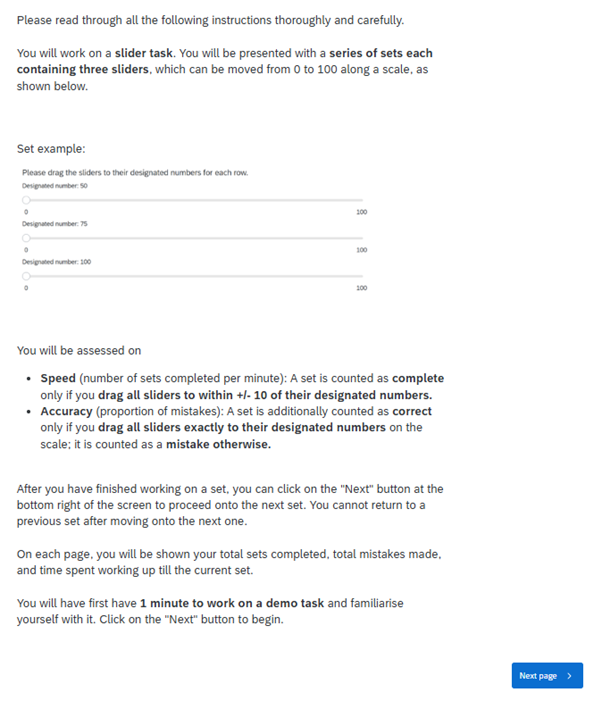
\includegraphics[width=\linewidth,height=0.9\textheight,keepaspectratio]{survey_screenshots/common_instructions.png}
\caption{Common instructions for all subjects}\label{fig:common-instructions}
\end{figure}

\begin{figure}[p]
\centering
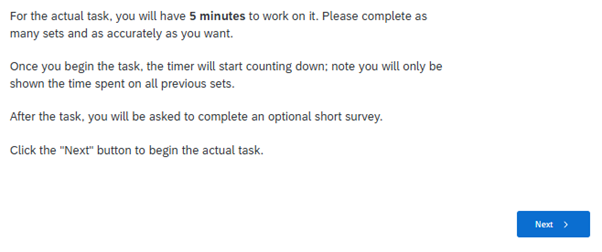
\includegraphics[width=\linewidth,height=0.9\textheight,keepaspectratio]{survey_screenshots/treatment1_instructions.png}
\caption{\Ctrl{} (Treatment 1) instructions}\label{fig:treatment1-instructions}
\end{figure}

\begin{figure}[p]
\centering
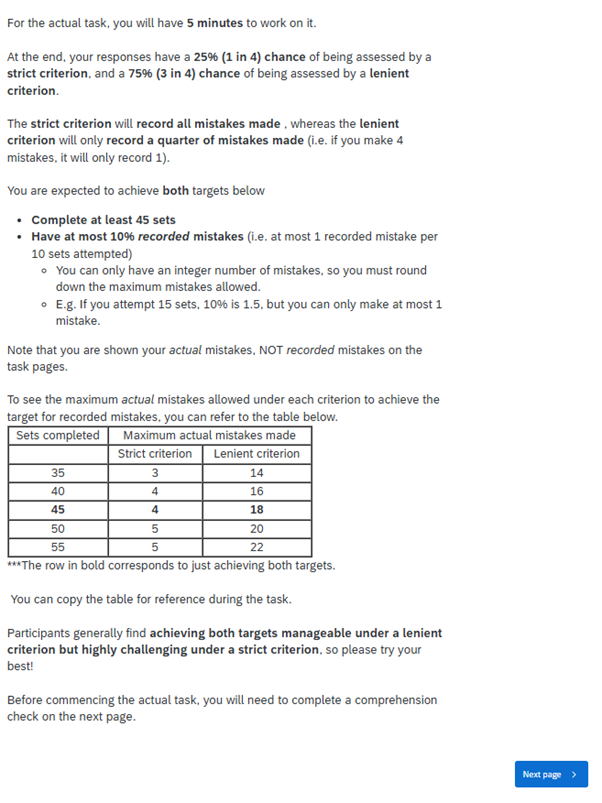
\includegraphics[width=\linewidth,height=0.9\textheight,keepaspectratio]{survey_screenshots/treatment2_instructions.png}
\caption{\LP{} (Treatment 2) instructions}\label{fig:treatment2-instructions}
\end{figure}

\begin{figure}[p]
\centering
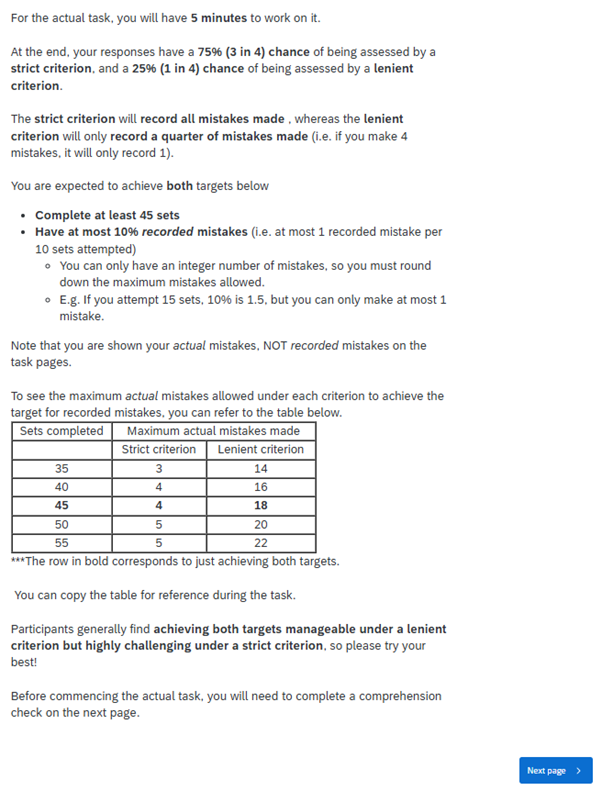
\includegraphics[width=\linewidth,height=0.9\textheight,keepaspectratio]{survey_screenshots/treatment3_instructions.png}
\caption{\SP{} (Treatment 3) instructions}\label{fig:treatment3-instructions}
\end{figure}

\begin{figure}[p]
\centering
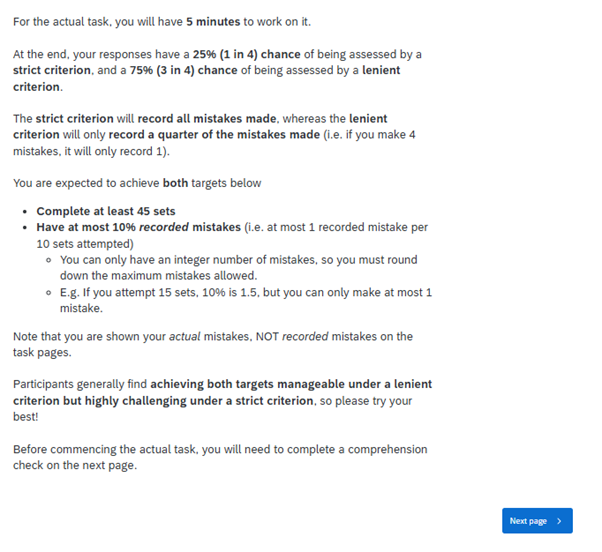
\includegraphics[width=\linewidth,height=0.9\textheight,keepaspectratio]{survey_screenshots/treatment4_instructions.png}
\caption{\LN{} (Treatment 4) instructions}\label{fig:treatment4-instructions}
\end{figure}

\begin{figure}[p]
\centering
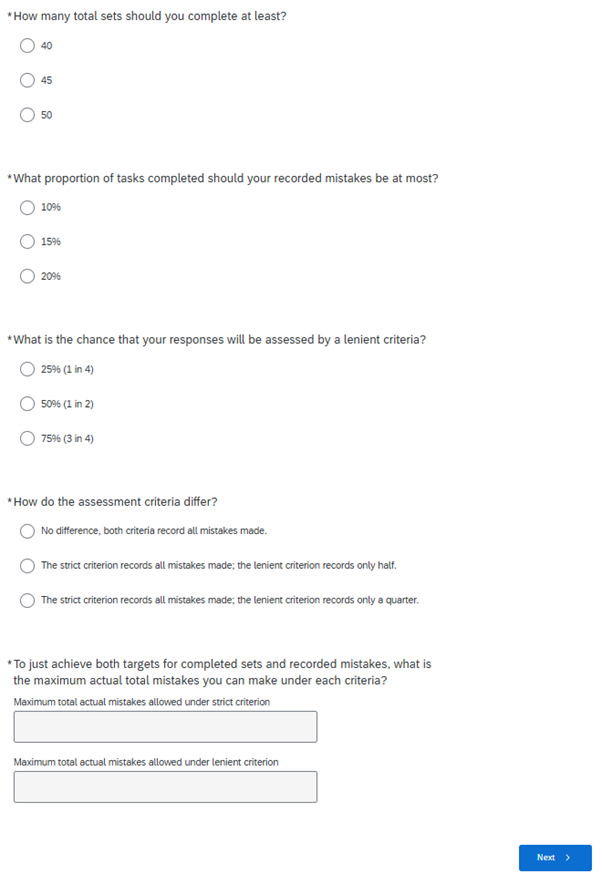
\includegraphics[width=\linewidth,height=0.9\textheight,keepaspectratio]{survey_screenshots/comprehension_check.png}
\caption{Comprehension check: last question only for \LP{} and \SP{}}\label{fig:compre-check}
\end{figure}

\begin{figure}[p]
\centering
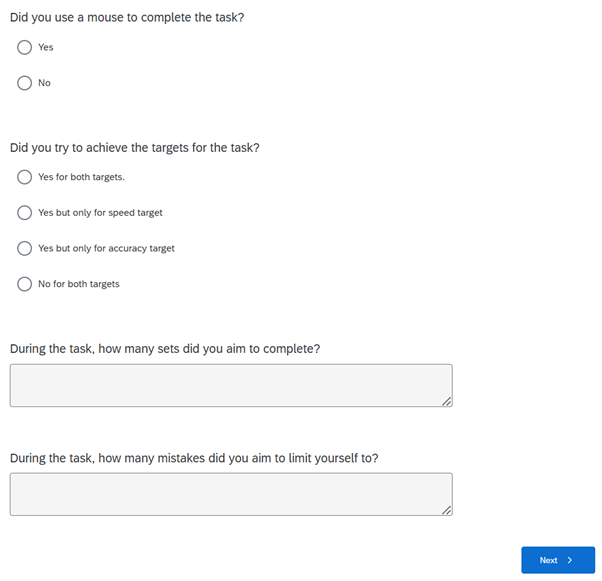
\includegraphics[width=\linewidth,height=0.9\textheight,keepaspectratio]{survey_screenshots/task_reflection_1.png}
\caption{Task reflection page 1}\label{fig:task-reflection-1}
\end{figure}

\begin{figure}[p]
\centering
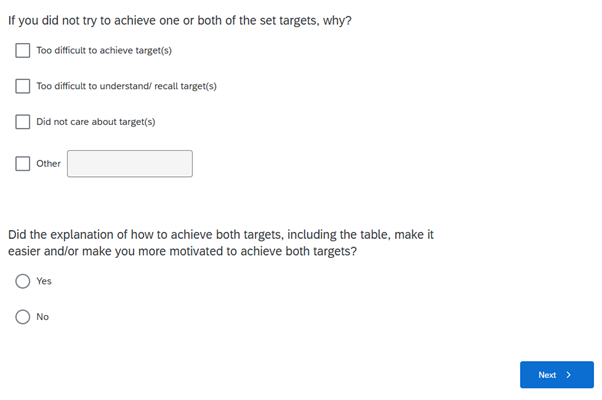
\includegraphics[width=\linewidth,height=0.9\textheight,keepaspectratio]{survey_screenshots/task_reflection_2.png}
\caption{Task reflection page 2}\label{fig:task-reflection-2}
\end{figure}

\begin{figure}[p]
\centering
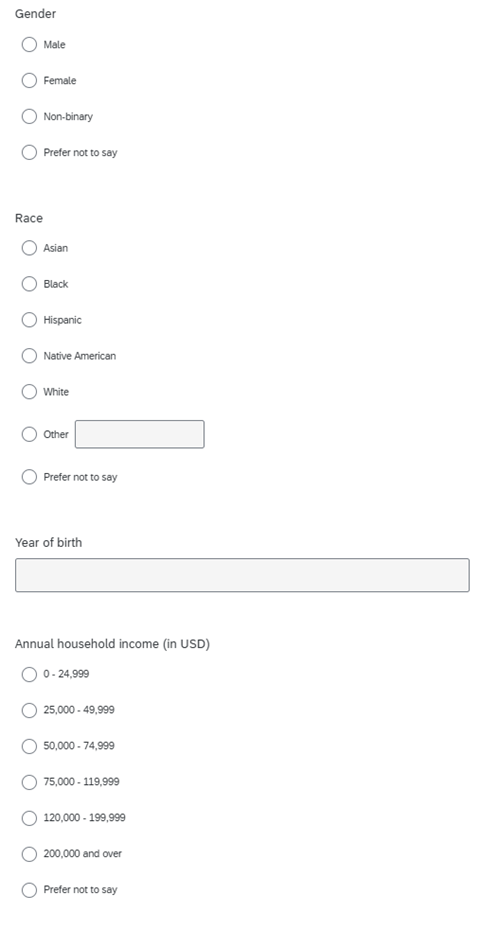
\includegraphics[width=\linewidth,height=0.9\textheight,keepaspectratio]{survey_screenshots/demographic_survey_1.png}
\caption{Demographic survey page 1}\label{fig:demographic-survey-1}
\end{figure}

\begin{figure}[p]
\centering
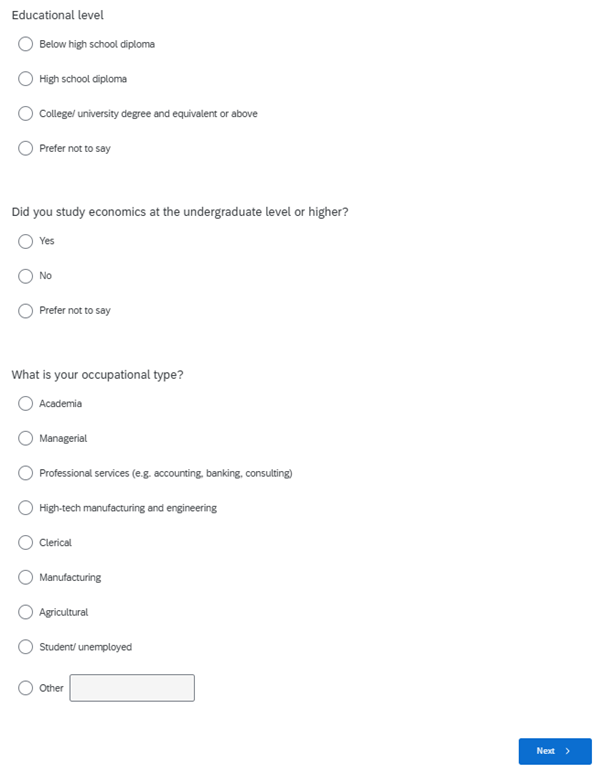
\includegraphics[width=\linewidth,height=0.9\textheight,keepaspectratio]{survey_screenshots/demographic_survey_2.png}
\caption{Demographic survey page 2}\label{fig:demographic-survey-2}
\end{figure}

\begin{figure}[p]
\centering
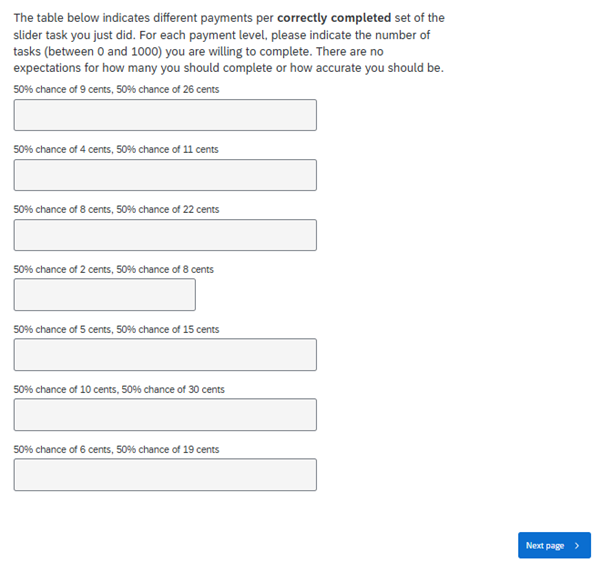
\includegraphics[width=\linewidth,height=0.9\textheight,keepaspectratio]{survey_screenshots/loss_aversion_survey_1.png}
\caption{Loss aversion survey page 1: pages and payment structures presented in random order}\label{fig:loss-aversion-survey-1}
\end{figure}

\begin{figure}[p]
\centering
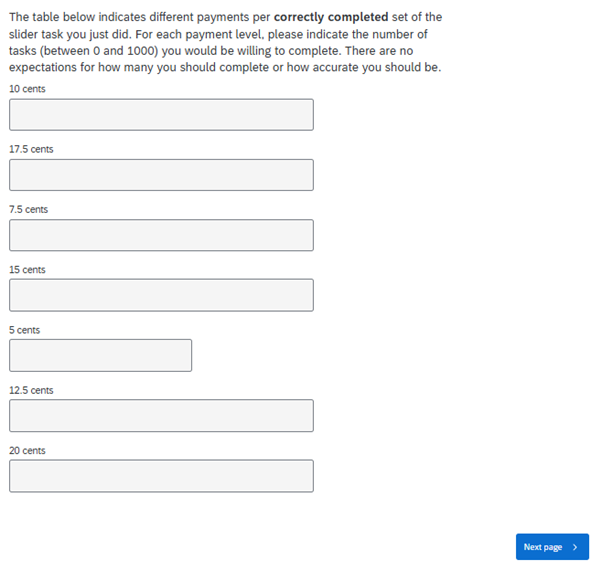
\includegraphics[width=\linewidth,height=0.9\textheight,keepaspectratio]{survey_screenshots/loss_aversion_survey_2.png}
\caption{Loss aversion survey page 2: pages and payment structures presented in random order}\label{fig:loss-aversion-survey-2}
\end{figure}

\end{document}
